\documentclass[a4paper,10pt]{article}

\usepackage[margin=2cm]{geometry}
\usepackage{graphicx}
\usepackage{hyperref}
\usepackage[all]{hypcap}
\usepackage{tabu}
\usepackage[title,titletoc,toc]{appendix}
\usepackage[english]{babel}
\usepackage{fontspec}
\usepackage[style=authoryear,backend=biber,sorting=nyt,dashed=false,urldate=long,abbreviate=false]{biblatex}
\usepackage{float}
\usepackage{fancyhdr}
\usepackage{microtype}

\addbibresource{references.bib}

\setlength{\headheight}{15.2pt}
\pagestyle{fancy}
\lhead{}
\chead{}
\rhead{\bfseries Software Requirements Specification}
\lfoot{Team Echo}
\cfoot{COS301 Software Engineering}
\rfoot{Page \thepage}
\renewcommand{\headrulewidth}{0.4pt}
\renewcommand{\footrulewidth}{0.4pt}

\setlength{\parindent}{0pt}
\setlength{\parskip}{1ex plus 0.5ex minus 0.2ex}

\frenchspacing

\title{
\includegraphics[width=12cm]{Eeufeeslogo.jpg} \\
       Software Requirements Specification \\ 
       and \\
       Technology Neutral Process Design \\
       Research Paper Management System \\
       \vspace{0.5cm}
       University of Pretoria \\
       \vspace{1.0cm}
       }

\date{} 
\author{Team Echo\\
	\vspace{0.5cm} \\
	\begin{tabu} to \textwidth { X[l] X[l]}
		\hline
		\textbf{Surname, First Name (Initial)}	& \textbf{Student Number}	\\ \hline \hline
		Bode, Elizabeth (EF)			& 14310156		\\ \hline
		Bondjobo, Jocelyn (JM)		& 13232852		\\ \hline
		Broekman, Andrew (A)		& 11089777		\\ \hline
		Loreggian, Fabio (FR)			& 14040426		\\ \hline
		Schutte, Gerome (GC)		& 12031519		\\ \hline
		Sefako, Motsitsiripe (MG)		& 12231097		\\ \hline
		Singh, Emilio (E)			& 14006512		\\ \hline
		\hline
	\end{tabu}}

\DefineBibliographyStrings{english}{%
urlseen = {\mbox{Accessed} on},
urlfrom = {[Online]},
in = {In},
}
\DeclareFieldFormat{url}{\bibstring{urlfrom}\space\url{#1}}
\DeclareFieldFormat{urldate}{\addcomma\space[\bibstring{urlseen}\space#1]}
\addto\captionsenglish{
  \renewcommand{\contentsname}
    {Table of Contents}
}

\begin{document}
\maketitle
\thispagestyle{empty}
\clearpage

\newpage
\pagenumbering{roman}
\thispagestyle{empty}
\tableofcontents
\clearpage

\newpage
\pagenumbering{arabic}

\section{Vision}
The client, Vreda Pieterse, from the University of Pretoria has requested a system to keep track of research publications in the Department of Computer Science at the University of Pretoria. The scope of the system is managing the administration involved in tracking of research publications within the department. However, collaboration on research papers is outside of the scope as a version control system is in use currently. The system is required to keep track of all publications and the associated metadata around the publications.

The department currently consists of various research groups, with various contributors, all producing research publications which should be tracked. As the University of Pretoria is rewarded for research produced, it is important for both the heads of research groups and the Head of Department to monitor the progress of current publications, and to gather other metrics to assist in other departmental planning.

The most important requirements as set out by the client are:
\begin{enumerate}
\item Monitoring the research output by the department through metrics by the Head of Department and heads of the research groups
\item Tracking the status of research publications
\item Being able to produce customized reports based on user defined values
\end{enumerate}

\section{Background}
This project was commissioned based on the following three problems faced by the client
\begin{itemize}
\item Limitations of current system:
	\begin{itemize}
	\item The current system used by the client involves utilizing one common Microsoft Excel spreadsheet document to keep track of the status of current research publications. A problem with this solution is that it causes data integrity problems due to the fact that it is not scalable.
	\end{itemize}
\item Increased productivity and transparency
	\begin{itemize}
	\item  A common issue faced by researchers in the Computer Science department is that an increased workload at due dates leads to the spreadsheet becoming unstable and subsequently crashing. Necessary data recovery on the spreadsheet leads to increased downtime, which, while also necessitating repeated data entry, decreases user productivity. Clearly, not a user friendly system, causing many a frustrated user.
	\end{itemize}

\item Monitoring and management of funding
	\begin{itemize}
	\item Currently the department receives funding based on research produced. The funding model, and hence, the amount, is based on various factors pertaining to the research publications, such as whether it is published, presented at a conference and so on. Therefore, having access to projections of the number and type of publications that are to be produced in coming years is very important for strategic departmental planning, as is monitoring historical performance of research groups and individual researchers.
	\end{itemize}
\end{itemize}

\section{Architecture requirements}
\subsection{Architectural scope}
At the very least, the software architecture should address the following responsibilities:
\begin{enumerate}
	\item Supply a persistence framework which
	\begin{enumerate}
		\item Relies mainly on databases.
		\item Supports integration with multiple databases and database technologies.
		\item Provides secure access to persistent data.
		\item Allows for importing and exporting of persistent data.
		\item Supports concurrent access.
	\end{enumerate} 
	\item Provide a reporting infrastructure, which is:
	\begin{itemize}
		\item Centralised.
		\item Independent of the rest of the functionality of the system.
		\item Consistent and accurate.
		\item Timely and reliable.
	\end{itemize}
	\item Allow for external access channels, which:
	\begin{enumerate}
		\item Supports system integration with front-end clients, the bare minimum of which should be a desktop web client and an Android mobile client.
		\item Work over a web protocol.
	\end{enumerate}
	\item Provide functionality benchmarking infrastructure.
	\item Provide integration with authentication frameworks.
	\item Cater for concurrent stateless access to services to at least fifty clients.
	\item Support system flexibility in adding or removing existing modules without necessitating system shutdown.
\end{enumerate}
\subsection{Access channel requirements}
\subsubsection{Human Access Channels}
The human access component must allow for both a desktop web client and an Android mobile client allowing the user to manage the metadata associated with research papers they are involved in. 

The web client will be the primary contact point for users of the system as most research papers are created, edited and maintained on personal computers that either owned by the contributor in question or the University of Pretoria. The web client will be based on an MVC based SPA architectural pattern. 

The Android application will be made available in the Android App Store to allow contributors to the system from outside the University of Pretoria to easily gain access to the system. The Android application should be accessible by all mobile devices running Android version 4.2 and upwards.

\subsubsection{System Access Channels}
All system access will be made over a uniform interface which will assist in faster development time, ease of maintenance and lower overall cost associated with the system. The common interface that will be used, will be a RESTful API based on the dissertation Architectural Styles and
the Design of Network-based Software Architectures of \textcite{fielding}.  All client side interaction will be done via the web client or Android application which will in turn use the RESTful API set of the system to accomplish the given task.

\subsection{Quality requirements}
\subsubsection{Performance}
\begin{enumerate}
\item \textbf{Description} \\
Application performance can be defined as the amount of work that can be accomplished by an application in question in a measured time interval. The time interval is normally measured in seconds, where the amount of work can be defined as the throughput, latency or data transmission time.
	\begin{itemize}
		\item \textbf{Throughput} \\
		The number of requests and responses which can be processed by the system in a given time interval.
		\item \textbf{Latency} \\
		A time interval measured as the time it takes to service a request. 
		\item \textbf{Data transmission time} \\
		The time it takes to transmit a request to the server from a client or a response from the server to the client. This is heavily influenced by the size of the request, as well as the quality of the network medium.
	\end{itemize}
	
	The aim for this system, is to increase the throughput and decrease the latency. As the developer has no control over the network medium used, he/she must aim for a minimal request and response payload as to decrease the data transmission time.
\item \textbf{Justification} \\
The current system suffers from performance issues, and hence, it is important for this new system to address these issues adequately. Our aim for this system is to increase throughput, decrease latency and data transmission time. This will ensure we have a system that is responsive at all times, including peak times and delivers an excellent user experience.
\item \textbf{Requirements}
	\begin{itemize}
		\item Network requests must be benchmarked, monitored and aggregate statistics about network requests must be made available.
		\item Function calls must be timed and benchmarked and this data should be logged.
		\item Precompiled SQL must be used in statements.
		\item Network responses should be cached on server side to lighten the load on database as well as decreasing the round trip time of request - response.
		\end{itemize}
\end{enumerate}

\subsubsection{Reliability}
\begin{enumerate}
\item \textbf{Description} \\
The design of this system is largely based on the fact that the current system used by the client is not reliable and suffers from system crashes and data loss. The newly designed system needs to be accessible from both inside University of Pretoria campuses as well as from other networks, especially on other campuses on the TENET network. The system should be reliable in both its accessibility and in the data that the system will use to calculate contributor metrics. 
\item \textbf{Justification} \\ 
The current system is largely unreliable in that it crashes under large workloads, and in that, because only one user can work on it at a time, many users get denied service during work critical times when workloads are high. This causes a detriment in user productivity. To ensure that the system can be used confidently as a tool to increase productivity and ease the work process, the development aim must be for the system to be as reliable and accessible as possible.
\item \textbf{Requirements}
	\begin{itemize}
		\item To enable offline activity and access of data from the Android app, data synced must be made differentiable with timestamps.
		\item The system must resolve synchronization conflicts using timestamps.
		\item Hot swapping of system modules should not affect system service reliability.
	\end{itemize}
\end{enumerate}

\subsubsection{Scalability}
\begin{enumerate}
\item \textbf{Description} \\
Scalability refers to the application in question's ability to handle an above normal workload for extended time periods and the mechanisms employed to facilitate this. The client has specified minimum conditions under which the system needs to function. However, the client has indicated that due to the business requirements, the system will experience higher workloads during the end of the month.
\item \textbf{Justification} \\
The system needs Scalability because it needs to support 10 research groups, with 100 members each working with 50 concurrent users. But these requirements may increase in future and hence the system should be able to handle additional loads.
\item \textbf{Requirements}
	\begin{itemize}
		\item The system should be able to handle 10 research groups with each research group containing 100 members.
		\item The system should be able to facilitate 50 concurrent user sessions at any time.
	\end{itemize}
\end{enumerate}

\subsubsection{Security}
\begin{enumerate}
\item \textbf{Description} \\
Security in application software refers to authentication, authorization, data security and accounting. Authentication refers to the systems' ability to provide a way of identifying a user, normally with a combination of a user name and password, or by using access tokens. Authorization refers to the systems' ability to determine whether the user in question has the required authority to execute certain commands or tasks. Data security refers to data only being accessible through authorised channels. Finally if the user has been authenticated and has the required authorization then accounting needs to be done to be able to determine how the users action has changed the system.  
\item \textbf{Justification} \\
Security is a important aspect of any software product. In terms of information security, we are concerned about integrity, availability, confidentiality and non-repudiation in that order. 

The reason we are most concerned about data integrity is that this data will be used to monitor and determine performance of researchers as well as assist in departmental strategic planning, which implies that the system must be available at all times to the heads of the research groups and the head of the department. 

Following this, is the aspect of data confidentiality, as we want to ensure passwords of the users stay secure as well as the metadata of research papers. The storing of metadata and subsequent leaking of this metadata can lead to other researchers publishing and patenting ideas first.

Finally, as this system is used to measure performance, it is important that non-repudiation of information is available, as researchers must be accountable for any information changes they make.
\item \textbf{Requirements}
	\begin{itemize}
		\item System should be resistant to SQL injections.
		\item A user group hierarchy system should be used to manage user access rights.
		\item Authentication credentials such as username and password should not be stored on Android user device. A token based authentication approach should be utilized so that only tokens are stored on end user device, allowing for the easy revocation of device access if a device is lost. Available technologies, such as OAuth, should be utilized.
		\item Password hosting with a unique salt for each user should be used.
		\item A key derivation function should be used with passwords. 
		\item After N invalid attempts, account should be locked for M min, where N and M would be agreed upon customer and developer based on current best practices.
		\item Database access must require authentication.
	\end{itemize}
\end{enumerate}

\subsubsection{Flexibility}
\begin{enumerate}
\item \textbf{Description} \\
Flexibility refers to the ability of the system to be changed dynamically either by hot swapping certain components in a live system or by extending the system with some kind of plugin. 
\item \textbf{Justification} \\
Flexibility is important for any system. A non-flexible system is restricted to using technologies that were hard coded into it, and this necessitates, at best, large scale refactoring every time an upgrade is available since new technologies need to be reintegrated, makes adding new features tedious, and risks the system becoming archaic. A flexible system requires minimum effort to upgrade and expand, allowing for the system to easily grow in usefulness and function beyond the original vision, and is directly in line with the requirement for the system to be cheap to maintain and upgrade, not just financially but also in labour. 
\item \textbf{Requirements}
	\begin{itemize}
	\item The system should allow unregistered users to use existing third party web service login credentials to register or log in to the service.
	\item The system should be decoupled from the database technology it uses and allow the client to select and change the database it uses in future.
	\item Authentication mechanisms used should be decoupled from the system, allowing them to be interchangeable.
	\item Modules should be decoupled from one another, allowing the system to be extensible without a break in service which is achieved by integrating new modules and swapping out existing ones. 
	\end{itemize}
\end{enumerate}

\subsubsection{Maintainability}
\begin{enumerate}
\item \textbf{Description} \\
The system is to be designed in such a way that it is easily updated, modified or extended by the client in the future. In order to achieve these requirements, design patterns and best practices such as coding style guides are normally used to ensure uniformity and modularity across the system.
\item \textbf{Justification} \\
Many systems require regular changes, not because they were poorly designed or implemented, but because of changes in external factors. For example we might need to update informations to meet the Computer Science laws and regulations.
\item \textbf{Requirements}
	\begin{itemize}
		\item All code should be documented in the applicable language documentation framework, such as JavaDocs for a Java based system, DOxygen for a C/C++ based system, etc.
		\item A coding style guide/manual should be set up and associated with the project, such that all developers use similar coding styles and conventions, to allow for more readable code that is easier to maintain.
		\item System should be separated in distinct, concise and independent modules relating to separate concerns, to allow for easier maintenance.
	\end{itemize}
\end{enumerate}

\subsubsection{Auditability/Monitorability}
\begin{enumerate}
\item \textbf{Description} \\
The system is to be designed to be verbose and transparent in its workings, and to ensure maximum data security, to allow role players to have insights into how the system is used and how it may be improved. These requirements are achieved by making the maximum amount of relevant data available to authorized users, logging performance critical information, and by enforcing strict constraints on the data that is stored. 
\item \textbf{Justification} \\
This is an important process in Software Engineering, where all the informations must be correct so requiring all the developers to see who made changes and when so that consistency must be kept in order to keep the database accurate and reliable.
\item \textbf{Requirements}
	\begin{itemize}
		\item Data in database should always be consistent. This implies that all data should adhere to constraints placed on the data by the data model, such as regex patterns, minimum and maximum length, non nullable fields, etc.
		\item No data should ever be deleted.
		\item It should always be possible to see which user created which objects at what time.
		\item It should always be possible to see which user last changed objects and at what time.
		\item An immutable log of user actions should be kept and should only be accessible by administrative staff.
		\item Logging of stack traces and crash analytics should be implemented in the mobile client, to ensure the developers can see to client reliability.
	\end{itemize}
\end{enumerate}

\subsubsection{Integrability}
\begin{enumerate}
\item \textbf{Description} \\
The system should allow for future external integration with other platforms such as security authentication providers, other external research meta-data databases etc.
\item \textbf{Justification} \\
The system necessitates integrability to allow for maximum usability, as the integrability of the system is directly related to how usable it is. To be usable, the system must allow for easy migration, not just from previous systems, but also to future systems and future data storage mediums. The usability is also largely determined by how well the back-end system integrates with front end clients, and which clients are supported.
\item \textbf{Requirements}
	\begin{itemize}
		\item The system should allow technology neutral importing and exporting of data.
		\item The back-end system should integrate with a desktop web client and Android mobile app clients.
		\item The system should be able to integrate with different back-end authentication services.
	\end{itemize}
\end{enumerate}

\subsubsection{Cost}
\begin{enumerate}
\item \textbf{Description} \\
The cost of the system entails any initial expenses as well as any ongoing expenses which the client may incur at some point. Such expenses arise from software licenses, external computing resources required as well as future maintenance of the system in terms of time.
\item \textbf{Justification} \\
The expenses made and software licenses cost must be taken into account in order to set the price of the software.
\item \textbf{Requirements}
	\begin{itemize}
		\item System should be cheap to operate, maintain and extend. If the quality and maturity of technologies available allow it, technologies used must be freely available/usable.
		\item As far as possible, open source compatible, mature technologies should be used, to ensure system stability as far as possible.
	\end{itemize}
\end{enumerate}

\subsubsection{Usability}
\begin{enumerate}
\item \textbf{Description} \\
Usability refers to ease with which humans, and to a lesser extent, servers, interact with the system in question. Usability can be measured in various ways such as using quantifiable scientific measures or more subjective measures with a key question point being if the API follows conventions and so on.
\item \textbf{Justification} \\
It is important that the new system is usable as it is a user-centric system. Ensuring that the system is usable will ensure that users capture accurate and correct information into the system which will for better performance and departmental strategic planning. As this system will also be used by parties outside of the Department of Computer Science of the University of Pretoria, it is important that the system conveys a professional image, as this will reflect on the image of the University of Pretoria. 
\item \textbf{Requirements}
	\begin{itemize}
		\item Each view in the desktop and mobile clients should be related to a single topic only.
		\item The web client should render properly and be fully functional in modern web browsers.
		\item Mobile devices running Android 4.2 and upwards should be fully supported.
		\item Material design UI guidelines prescribed by Google must be used, to ensure that the clients feel modern and familiar. 
		\item Android app and web client should support the full back-end API specifications.
		\item The user must be allowed to elect whether they would like their data to be available offline.
		\item Mobile client users should be able choose between downloading data over Wi-Fi or 3G. 
	\end{itemize}
\end{enumerate}

\subsection{Integration requirements}
The web interface should be accessible to most modern PCs with a modern browser. The website will be making use of an SPA MVC based design which will query a RESTful API, resulting in a very light, mobile and responsive web interface that will it to work across various devices.

The Android application will be built to work on all Android version 4.2 and upward devices. The mobile application on the Android device should be sensitive to the amount of data that is transmitted over the network due to the high cost of mobile internet in South Africa. To allow for minimal communication but maximum functionality, the MVC based design will be followed in the Android application design.  Furthermore, the use of accessing RESTful APIs will allow objects to be transmitted on the wire with a very minimal representation, thereby saving on client bandwidth costs.

The RESTful API will be implemented using the HTTP protocol as a high level protocol. The reason that HTTP is chosen is that it is a widely supported and deployed protocol, allowing a lot of flexibility. Furthermore, most JavaScript libraries, and the Android platform itself, have excellent support for RESTful APIs over HTTP.

\subsection{Architecture constraints}
The architectural constraints are used to improve the architectural analyses of quality characteristics of the software to be developed. Our system architecture will be based on the following system architecture and technologies which will be used:

\begin{enumerate}

	\item \textbf{Representational State Transfer  (REST)}
	REST which depends on stateless client server and communications protocols, and uses the HTTP protocol in most cases. It is an architectural style used to design networked applications. All the four CRUD operations are used in REST. 

	\item \textbf{Service Oriented Architecture (SOA)}
	SOA makes it easier for software components on computers that are connected on a network to work together with no need to make changes to the underlying program itself. The concept of service is what SOA is based on.

	\item \textbf{Frameworks} 
	Frameworks are a special case of software libraries in that they are reusable abstractions of code wrapped in a well-defined API. Here are a few that our system will use:
	
	  \begin{itemize}
		  \item The Spring framework: is a technology that is associated with developing secure websites and interacting with databases in conjunction with Hibernate. Spring is simply a usable API, with the idea being for the developer to represent Java objects with Spring Beans.
		  It is an inversion of control container which is just a configuration of application components and life-cycle management of Java objects, it is usually done though dependency injection. Spring is especially an application framework for the Java platform. 
		  \item Liquibase: allows tracking, management of database schema changes to relational object databases.
		  \item Apache Log4: allows total control over log statements that are output. The system's configuration is available at run-time using external configuration files, fulfilling the quality requirements of flexibility and auditability.
		  \item Hibernate ORM: provides various a feature such as SQL generation and is an object relational mapper framework for Java, which allows the mapping of Java classes onto relational database tables.
		  \item Java Jersey: provides RESTful web services for Java.
	  \end{itemize}
	
	Any Java application can use the framework's core features , but for building web applications on top of a Java Enterprise Edition platform some extensions exists. Even though, the framework does not impose any specific programming model. 
	Therefore, spring can helps us achieve integrability and maintainability by using design patterns and any programming model to ensure uniformity across the system.
	
	\item \textbf{Dependency Injection (DI)}
	DI will eases software testing and re-usability of software by using a design based on independent classes/components thus achieving the usability requirement.

	\item \textbf{Unit Testing}
	Unit Testing to automate the following tasks: compilation of Java source code, running test cases and generating project documentation. It will be used as well because it gives us the following benefits
		\begin{itemize}
			\item Reduced system failure risk,
			\item Rapid feedback on developed components,
			\item Improved Maintainability due to unit testing,
			\item Improved Re-usability leading to less code being developed and maintained.
		\end{itemize}
		
	\item \textbf{Programming language}
		\begin{itemize}
		\item HTML
		We will build a browser based SPA.
		\item JavaScript\\
		JavaScript will make out the core of the SPA.
		\item CSS\\
		We will use this to implement the styling of the application.
	\end{itemize}
	\item \textbf{Operating system}
	The system will be deployable on Windows, MAC and UNIX operating systems as well as Android devices.
\end{enumerate}
\subsubsection{Architectural Patterns}
	\begin{itemize}
		\item \textbf{Authentication Enforcer Pattern} \\
		The authentication enforcer pattern is focused to provide a centralized managed authentication mechanism, to verify the identity of users and encapsulating the details of authentication. This patterns assist in removing security checks from business logic code, thereby providing cleaner, more robust and easier to maintain code.
		
		Further, since authentication is centralized, this pattern further allows changes to be easily implemented in terms of the authentication procedure, such as using a different authentication flow, or even mechanism, such as authenticating the user against an external provider.
		
		\subitem \textbf{Reasons for selecting this pattern:}
		\begin{itemize}
			\item Since this pattern enforces separating security modules from business logic modules, it contributes to the reliability of the system by making it easier for system modules to be swapped without affecting system reliability. As long as the authentication mechanism provides the same service to the system, it can be easily exchanged with or upgraded to a different module which provides a similar service.
			\item This pattern lends itself well to integrating separate existing technologies into the system. This allows the developer to choose an existing technology which supports token based authentication as per the requirements.
			\item A pattern requiring a separate security module satisfies the flexibility requirement that authentication mechanisms must be decoupled and interchangeable, and this lends itself well to system maintainability, as well as system integrability.
		\end{itemize}
	
		\item \textbf{Authorization Enforcer} \\
		Similar to the authentication enforcer pattern, this pattern provides a centralized managed authorization mechanism, thereby abstracting authorization code away from application code.  With this pattern, it assists the system in authorizing users, i.e. to determine whether the current user has the required roles or privileges to perform a certain action. All of the benefits referred to in the authentication enforcer pattern are also applicable here, and the reasons for choosing this pattern remains the same.
	
		\item \textbf{Client-Server Architectural Pattern:}\\
			A network technology in which each computer connected on the network is either a server or client is called a client server architecture.
			\begin{enumerate}
				\item Servers: are powerful computers which are used to process the client requests.
				\item Client: is simply a computer connected on the network which is used to send request for some resources to the server.
			\end{enumerate}
			Requirement of client server: It models work in a networked environment therefore the processing of an application distributed between the client and the server.
			Function of client server: An interface/form is provided by the client to allow a user to request services of the user and to display the results the server returns.
			
			Client-Server Architectural Pattern is used because we need to have reliability on the system. Data can be retrieved for further processing from any computer connected on that network.
		
		\subitem \textbf{Reasons for selecting this pattern:}
		\begin{itemize}
			\item This pattern allows decoupling of business logic- and human adapter modules, adhering to the maintainability and flexibility requirements.
			\item It enables system usability by not requiring users to incur large downloads to make use of the system.
			\item The pattern lends itself well to maintainability, since developers are able to upgrade and fix problems in the system module without affecting the front-end, and vice versa.
		\end{itemize}
		
		\item \textbf{Layered Architectural Pattern:}\\
		A design pattern in which software is divided up into individual layers by functionality. The layers interact with one another via requests and responses, and there are typically four of these layers:
		\begin{enumerate}
			\item Presentation/view: The user interface that the user interacts with, such as a desktop client.
			\item Application/controller: The service API that the presentation layer interacts with in order to perform system functions.
			\item Business logic: The functions that get called by the service API, to interact with system data.
			\item Data access: The layer that provides data access to the business logic layer 
		\end{enumerate}
		
		This pattern is used because it lends itself well to decoupling software modules from one another, and allows for separation of concerns. At the very least, the view layer is decoupled from the business logic, and the controller layer is decoupled from the data access. Furthermore, when each layer object realises a contract, all layers are completely decoupled from one another, and allows for layer objects of the same layer type to be interchanged without any hassle. 
		
		\subitem \textbf{Reasons for selecting this pattern:}
		\begin{itemize}
			\item The concern of caching network responses can be separated from the other layers in the pattern.
			\item The pattern enables trivial swapping of groups of modules which satisfies the reliability, flexibility, integrability and maintainability quality requirements.
			\item The pattern allows decoupling the database and authentication modules from the rest of the system as per the maintainability requirements.
		\end{itemize}
		
		\item \textbf{Representational State Transfer (REST) Architectural Pattern:}\\
		REST is an architecture pattern for designing networked applications. The idea is instead of using complex mechanisms such as SOAP, CORBA or RPC to connect between machines or to make calls between machines, simple HTTP is used.
		
		The Uniform interfaces which is combined of resource names and HTTP, GET, DELETE, POST, PUT.
			A REST service is:
		\begin{enumerate}
			\item Language-independent (C\# can communicate to Java, etc.),
			\item Can be used with firewalls,
			\item Platform-independent (MAC, Windows, UNIX) and,
			\item Standards-based (runs on top of HTTP)
		\end{enumerate}
		
		\subitem \textbf{Reasons for selecting this pattern:}
		\begin{itemize}
			\item Using the REST pattern allows for system flexibility since it enables platform independent communication between business logic- and human adapter modules.
			\item The pattern satisfies maintainability- and cost quality requirements, since it being language independent allows easy migration of services to different technologies while keeping communication methods well defined.
			\item It enables the integrability quality requirement to integrate the service with an Android mobile client and a desktop web client, by defining a communication mechanism between the clients and the server.
			\item REST network responses can be cached, satisfying the performance quality requirement.
		\end{itemize}
		
		\item \textbf{Secure Data Logger Pattern} \\
		A requirement stated by the client is that the proposed system should contain a full audit trail functionality, which would allow administrators to view any action that executed by users, as well as the modification that execution had on the data.
		
		For this requirement the Secure Data Logger Security Pattern can be utilized. This pattern aims to log application system log to a secure tamper-proof log system, which would prevent users from modifying the audit trail. This pattern also goes further by ensuring the integrity of the log message, which can be achieved by various means, such as cryptographically signing the message, or encrypting the message before it is sent to the store.
		
		This pattern provides two important security features, depending on how the logging system, as well as the message are secured in the system.  The first protection, is that should a malicious user gain access to the logging system, they will be unable to use the data to plan further attacks on the system.  The second protection provided by this pattern, is that any modification of the log data will be detectable by administrators.
		
		\subitem \textbf{Reasons for selecting this pattern:}
		\begin{itemize}
			\item The pattern can be applied in such a manner that timestamps of actions taken using the service might be more auditable, increasing system reliability.
			\item The pattern satisfies the security quality requirement by making log messages tamper proof and disallowing users to modify the audit trail.
			\item By keeping a log of actions committed by users, such as creation and modification of objects, and storing these in an immutable log, this pattern satisfies the auditability quality requirement.
		\end{itemize}
		
		\item \textbf{Services Orientated Architecture/ Microservices Architecture:}\\
		An architectural pattern in software design in which system use cases are divided into one or more service operations, and these service operations are then implemented, either individually or combined with other service operations, by a reusable SOA service. The SOA architecture itself comprises five layers:
		\begin{enumerate}
			\item Consumer interface: The GUI for end users accessing application services
			\item Business process: The representation of system use cases
			\item Services: The consolidated inventory of all available services.
			\item Service components: The reusable components used to build the services, such as functional libraries.
			\item Operational system: Contains data repository, technological platforms, etc.
		\end{enumerate}
		Not to be confused with an API, this architectural pattern provides an aggregated collection of services which implement the use cases of the system. The user or developer themselves can choose which of these available services to call on. This architectural pattern was chosen because it is built around the principles of decoupling modules. Service objects must be decoupled from one another and can be distributed on different machines and implemented using different technologies, but implement a single interface, and communicate with one another using well defined interfaces, either locally or over a network. This also lends itself well to system reliability and scalability. More than one system provider may be used, enabling the system to switch to another service provider should one fail, or instantiating more service providers if system load increases. This pattern satisfies all the same quality requirements as the layered architecture pattern.
	\end{itemize}

\section{Architectural tactics or strategies}
\subsection{Software Engineering Context : Architectural Tactics}
Achitectural tactics is concerned with achieving coherence between  a design decision and a quality response/promise. So by definition, Architectural Tactics are points of leverage for achieving quality attributes previously stated in the requirements section - simply put, this referes to how we plan to keep our promise of the level of quality stated previously. 

\subsection{Performance Tactics}
	\subsubsection{Performance Tactics can be divided into 3 groups}
		\begin{enumerate}
			\item Tactics for managing resource demand : these tactics control execution and transfer times by controlling the allocation of resources
			\item Tactics for managing conflict resolution : these tactics control pre-emeption and waiting times when competing requests execute concurrently. 
			\item Tactics for managing multiple resources : these tactics enable multiple resources to be used efficiently to ensure that available resources are allocated upon request. 
		\end{enumerate}

	\subsubsection{In context of the system}
		\begin{itemize}
			\item Precompiled SQL must be used in statements.\\
				The system is designed to handle concurrent requests. The use of threads will be crucial in the pre-compilation of SQL statements to increase performance. During compilation, multiple threads will run ahead and compile the SQL statements, and as threads complete their execution, the process will be ready to handle the request from the user(s) and provide a timely response. 

			\item Network responses should be cached on server side to lighten the load on database as well as decreasing the round trip time of request-response.\\
				This will increase the number of requests and responses the system handle in an interval of time. This will rely on a server that is designed to store data and information likely to be requested next. This will also obviously drastically reduce computational overhead during executions. 
			\item Function calls must be timed and benchmarked and this data should be logged."+ "Function calls must be timed and benchmarked and this data should be logged.\\
				The server will log metadata pertaining to each function call and network request, and in further development of the system, developers will use this information to tweak the efficiency of requests and thus, improve the systems current performance. 
		\end{itemize}

\subsection{Reliability Tactics}
	Reliability of the system refers to amongst other things, the coherence of information stored within the system and presented to users(concurrent). This can be achieved through the use of a duplication scheme which can be sought after using Passive Redundancy, which simply means that the system is designed to store the same information multiple times in multiple independent locations. 

	System reliability also refers to the systems automatic fault detection. 

	\subsubsection{In context of the system} 
		\begin{itemize}
			\item To enable offline activity and access of data from the Android app, data synced must be made differentiable with timestamps."\\
				\begin{itemize}
					\item This will be achieved by providing persistent data storage services with state information, ensuring that the results obtained - either using the Android application or the website is still valid.  
					\item A variation of the Blackboard Architectural pattern will be used to define checkpoints which allow for roll back functionality. All inputs into the system will be logged in order, in this way, should an inconsistency occur, one could reconstruct the sequence of events. 
				\end{itemize}
			\item The system must resolve synchronization conflicts using timestamps.
				\begin{itemize}
					\item The Ping/Echo Architectural tactic will be used to achieve this requirement. 
					\item It has two major components ; the one issuing the ping and keeping time and the components responding to the ping with an echo. 
					\item The sequence of actions is controlled by a clock, independent of all the other actions in the system. 
					\item Another way this requirement will be fulfilled is through the use synchronization locks (which ensure that only one process at a time can make use of a shared resource) on all critical sections of the system, processes must attempt to acquire a lock before they can use a shared resource and release the lock once they are done using the resource.
					\item Voting tactic will be used for conflict resolution here : different components work on the same problem, their results are compared and the voting scheme is used in cases where results differ.
				\end{itemize}
			\item Hot swapping of system modules should not affect system service reliability.
				\begin{itemize}
					\item The Broker Archictectural Pattern will be used here because it maintains communication with the server. Since it adds timing behaviour, it can be used to roll back events to repaire the system should it be affected by hot swapping of system modules. 
					\item The system will not suffer much strain since it is designed using the MVC model, only some modules would be affected but detection and repair is made easy because the system will be made up of separate individual modules. 
					\item Hiding information : modules of the system will have their responsibilities divided into two categories - public and private. This will limit responsibility as well as dependency so one module failing will not affect the others by a huge margin. 
				\end{itemize}
		\end{itemize}


\subsection{Scalability Tactics}
	\subsubsection{Definition of Scalability}
		\subparagraph
		- Scalability refers to the ability to handle increased workload without adding more resources to the system.
		- One way to achieve scalability is to perform a regular SWOT analysis on the system: 
		--Strengths : the kinds of growth the system is designed to handle 
		--Weaknesses : the kinds of growth the system will have trouble handling
		--Opportunities : possible changes in the system which could be exploited to increase performance 
		--Threats : possible changes in the workload that the system will not be able to handle

	\subsubsection{In context of the system}
		\begin{itemize}
			\item The system should be able to handle 10 research groups with each research group containing 100 members.
				\begin{itemize}
					\item Developers need to be aware of the systems abilities at all times, this will be achieved through regular Scalability Audits. 
					\item If demand never reaches a critical level, the incremental cost for scalability will be wasted because designing a system to be scalable may entail upfront costs that are higher than those of a less scalable version of the same system. 
				\end{itemize}
			\item The system should be able to facilitate 50 concurrent user sessions at any time.
				\begin{itemize}
					\item Centralized control leads to resource bottlenecks, which is not favoured favoured especially since 50 concurrent users should be able to use the system concurrently.  
					\item Decentralising control to allow multiple users to act on the system at a time, more especially if their processes are not executing critical regions is an Architectural tactic which will allow multiple users to act independently on the system. 
			\end{itemize}
		\end{itemize}

\subsection{Security Tactics} 
	Security refers to ensuring that only permitted people are allowed to access and modify the system in any way. Access needs to be controlled and monitored, and levels of access need to predetermined such that a normal user has more restrictions than a super user. 

	\subsubsection{In context of the system :} 
		\begin{itemize}
			\item System should be resistant to SQL injections.
				\begin{itemize}
					\item Encrypting data is one measure which will be used to prevent SQL injections. SQL injections rely on knowing what type of data is expected, if this data is encrypted when it gets to server and turned into something only the system will understand, then a SQL injection attack can be avoided. 
					\item The system never stores authentication information as simple text. 
				\end{itemize}
			\item A user group hierarchy system should be used to manage user access rights.
				\begin{itemize}
					\item The different types of actors on the system will have different access rights, this will be accomplished by disabling some functionality and modules depending on the level of user that logged in. 
				\end{itemize}
			\item Authentication credentials such as username and password should not be stored on Android user device. A token based authentication approach should be utilized so that only tokens are stored on end user device, allowing for the easy revocation of device access if a device is lost. Available technologies, such as OAuth, should be utilized.
				\begin{itemize}
					\item OAuth will be used to achieve this requirement. 
					\item OAuth is an authorization framework which enables a third-party application to obtain limited access to an HTTP service. 
					\item OAuth is serves as a simple mechanism to publish and interact with protected data. 
				\end{itemize}
			\item Password hosting with a unique salt for each user should be used.
				\begin{itemize}
					\item This security feature will be implemented using hashing. When the user creates their account, their password will automatically be hashed and stored in the database in its hashed version, it is never stored in plain-text. Each time the user logs on, the hashed version of the password will be queried, instead of the plain text version. 
				\end{itemize}
			\item A key derivation function should be used with passwords.
				\begin{itemize}
					\item This functionality will happen during hashing of the password before it is stored persistently. 
				\end{itemize}
			\item Database access must require authentication.
				\begin{itemize}
					\item The level of access and ability to view or modify any database linked to the system will be determined by the type of user logged into the system. 
					\item User authentication will be performed using Access Tokens, which will be checked for validity every time a database is queried. 
				\end{itemize}
		\end{itemize}


\subsection{Flexibility Tactics}
	The following Flexibility tactics will be used to ensure that the system can handle dynamic, run-time changes. The tactics used also for allow for plugability which can be used to extend the functionality of the system. 
	
	\subsection{In context of the system}
		\begin{itemize}
			\item The system should allow unregistered users to use existing third party web service login credentials to register or log in to the service.
				\subparagraph
					- StrongLoop (An IBM product) is an API framework which will be used to allow users to register and login to the system using their credentials from their Facebook, Google, Twitter or Github accounts.
			\item The system should be decoupled from the database technology it uses and allow the client to select and change the database it uses in future.
				\subparagraph
					- This functionality will be achieved by converting database tables to XML. As long the structure and data of the database is maintained, the XML version can be converted back into a database - this allows the information to be preserved in the new database too. 
					- IBM DB2 XML Extender will be used in this regard to store  XML documents as BLOB-like objects or as a decomposed set of tables. 
			\item Authentication mechanisms used should be decoupled from the system, allowing them to be interchangeable.
				\subparagraph
					-This quality requirement will be achieved using The Pluggable Authentication Modules(PAM) library, which is a generalised API for authentication-related services. This API allows the system developer to add new authentication methods by simply installing new PAM modules. This will give the system the ability to add and remove authentication mechanisms. 
		\end{itemize}


\subsection{Maintainability Tactics}
	Maintainability Tactics allow the existing software/ system to be modified while preserving its integrity. 
		
	There are four categories of Software Maintenance
	\begin{itemize}
		\item Adaptive : changes in the software environment 
		\item Perfective : new user requirements 
		\item Corrective : fixing errors 
		\item Preventative : preventing future problems
	\end{itemize}
	
	\subsubsection{In context of the system} 
		\begin{itemize}
			\item All code should be documented in the applicable language documentation framework, such as JavaDocs for a Java based system, DOxygen for a C/C++ based system, etc.
				\begin{itemize}
					\item Doxygen will be used for code documentation since it supports a variety of programming languages such as Java, C\#, and PHP. 
				\end{itemize}
			\item A coding style guide/manual should be set up and associated with the project, such that all developers use similar coding styles and conventions, to allow for more readable code that is easier to maintain.
				\begin{itemize}
					\item Simple good coding practices known by all system developers should be used. These include camel casing and giving descriptive names to variables, functions and classes. 
				\end{itemize}
			\item System should be separated in distinct, concise and independent modules relating to separate concerns, to allow for easier maintenance.
				\begin{itemize}
					\item The Spring framework is used for this quality requirement because it supports seperating the different modules of the system so that they can be tested as independent modules. 
					\item Spring also supports transaction management which unifies several transaction management APIs and co-ordinates transactions for Java objects.
				\end{itemize}
		\end{itemize}

\subsection{Auditability Tactics}
	These tactics are used to ensure that information about the performance of the system is always available, and to provide a log of which user provided which input at which point in time. 
	
	\subsubsection{In context of the system}
		\begin{itemize}
			\item Data in database should always be consistent. This implies that all data should adhere to constraints placed on the data by the data model, such as regex patterns, minimum and maximum length, non-nullable fields, etc.
				\begin{itemize}
					\item Data validation will be enforced by the developer on the client side, this will ensure that only valid data will be entered into any database associated with the system. 
 					\item RegEx(Regular Expressions) Patterns will be used to ensure that any input into the system is of the right format. 
				\end{itemize}
			\item No data should ever be deleted.
 				\begin{itemize}
					\item This will be accomplished by not adding any functionality that gives regular users to remove records from the system. The only way to 'delete' information from the system is to render it unusable - by disabling access to it - a feature which must be enforced by the developer.
				\end{itemize}
			\item The rest of the quality requirements pertain to logging of system actions.
				\begin{itemize}
					\item his requirement will be succeeded by externally logging all inputs and actions by the user by having the system write them to a text file. 
					\item Logging system data will not be a user function. Logging happens automatically by the system, without the user being aware or able to intercept the process.
				\end{itemize}
		\end{itemize}

\subsection{Integrability and Extensibility Tactics}
	\subparagraph
		- Integrability evaluation refers to testing whether separately developed components work together correctly.  Extensibility evaluation focuses on how new features can be added without losing existing features

\subsubsection{In context of the system} 
		\begin{itemize}
			\item The system should allow technology neutral importing and exporting of data.
				\begin{itemize}
					\item The design of the database will allow the information stored to be easily converted to XML format, this makes it easy to export the information stored in the tables to be used by another technology. 
				\end{itemize}
			\item The back-end system should integrate with a desktop web client and Android mobile app clients.
				\begin{itemize}
					\item This requirement will be fulfilled through the use of Hybrid. Hybrid has two main components, native code (Java and Android frameworks) and web code (HTML/CSS/JavaScript). This will give us a web interface which can easily be bundled as an Android Application. 
				\end{itemize}
		\end{itemize}


\subsection{Cost Tactics} 
	\subsubsection{In context of the system}
		\begin{itemize}
			\item System should be cheap to operate, maintain and extend. If the quality and maturity of technologies available allow it, technologies used must be freely available/usable.
				\begin{itemize}
					\item As it is, no special technology is required by the user to interact with the system. The user only needs a device to access the system. 
				\end{itemize}
			\item As far as possible, open source compatible, mature technologies should be used, to ensure system stability as far as possible.
				\begin{itemize}
					\item Free Open Source software will be used to build the entire system. The only thing required when writing web pages is a text editor and a web browser to view the pages. NetBeans is a free IDE which can easily be acquired and used without a product key. 
				\end{itemize}
		\end{itemize}


\subsection{Usability Tactics}
	\subsection{In context of the system}
		\begin{itemize}
			\item The web client should render properly and be fully functional in modern web browsers.
				\begin{itemize}
					\item  One way the system will achieve the optimization of web page rendering is that while running javascript code, browsers cache the changes and apply them in a single pass after the code was run. 
					\item Always use the (\#id) selector for CSS because it is the fastest and will optimize rendering of the Cascading Style Sheets. 
				\end{itemize}
			\item Mobile devices running Android 4.2 and upwards should be fully supported.
			\item Android app and web client should support the full back-end API specifications.
				\begin{itemize}
					\item  This quality requirement will be taken care of automatically by Hybrid(as mentioned above.
				\end{itemize}
		\end{itemize}


\section{Reference architectures and frameworks}
\subsection{Backend System}
\subsubsection{Programming Languages}
	\begin{itemize}
		\item Java
			\subparagraph{Description}
			Java in this instance refers to the programming language. Java is an object-oriented language that supports concurrency and classes. 		\subparagraph{Performance}
			The reader may note that historically, Java has been considered to have worse performance than languages such as C and C++. Primarily, this is due to the fact that Java programs run on the Java Virtual Machine as opposed to the computer's processor. However, to assay those fears, the performance of Java in recent versions has improved dramatically by the use of the Just-in-Time compilation. Combine this with the ability to compile Java code once and then run the program without recompilation on a different computer, means that Java is still an ideal contender for a programming language for use in the system.
					\subparagraph{Scalability}
			When referring to the Scalability requirement, Java has relatively high performance when used for High Performance Computing, HPC, and is similar to Fortran on the more intensive benchmarks. However, there does exist a scalability issue for the Java Virtual Machines to perform intensive communication on grid networks. To again assay fears of viability in this system, much of the scalability issue with Java Virtual Machines lies in the hardware setup and not on the software side.		
				
			\subparagraph{Flexibility}
			For the Flexibility requirement, Java excels as it operates on the WORA or Write Once, Run Anywhere principle. Java code can run on all platforms that support Java without the need for a recompliation. This is accomplished via the fact that Java applications are compiled to bytecode. This bytecode can run on any Java virtual machine and is totally independent of the computer architecture. This means that Java code, once writtten, can be easily and quickly ported and deployed throughout the various system components.


			\subparagraph{Cost}
			The latest version of Java is Java 8 which is supported for free by Oracle meaning that its use in this system does not contribute towards system cost.
			\subparagraph{Usability}
			From a programming perspective, Java offers a number of features that make it an adaptable and useful language for programming. One of the core features is that Java provides an automatic memory management service or automatic garbage collector. This means that the programmers are freed from the concerns and complexities of memory management, and the contiguous issues associated therein.

			From a syntactical perspective, Java offers a similar syntax to 
			Frameworks C and C++ meaning that learnability of Java is typically much lower, especially with the use of IDEs such as Netbeans or Eclipse.
\end{itemize}
\subsubsection{Frameworks}
	\begin{itemize}
		\item Spring Framework
			\begin{itemize}
				\item \textbf{Description}\\
					The Spring framework is an application framework and inversion of control for the Java platform, built on top of Java EE
				\item \textbf{Performance}\\
					Performance of a framework cannot be quantified with a number, but rather in respect to its components. Spring framework is a widely used framework that is seen as a replacement for Java EE. Therefore we can say that Springs performance is at a high level.
				\item \textbf{Reliability}\\
					The Spring framework is reliable in the sense that it makes the programmer code less, and do more. Thus having less logic errors the system will be more reliable
				\item \textbf{Scalability}\\
					Spring framework is designed for scalability and with Java as the language of choice, its scalability is increased.
				\item \textbf{Security}\\
					Spring framework has Authentication and Authorization modules which provide good security of data.
				\item \textbf{Flexibility}\\
					Spring framework provides many independant modules which are hotswappable, thus it is is flexible.
				\item \textbf{Maintainability}\\
					There are many package/dependancy managers that are available for Spring that keeps all code the latest.
				\item \textbf{Auditablility/Monitorability}\\		
					Spring audits all events and one can view these stats.
				\item \textbf{Integrability}\\
					Spring has its own integration framework that provides reusable functions.
				\item \textbf{Cost}\\
					Spring is opensource.
			\end{itemize}
			
		\item Spring Boot
			\begin{itemize}
				\item \textbf{Description}
				Spring boot is a convention-over-configuration solution for creating stand-alone, production grade Spring based applications that you can just "run"
			\end{itemize}
			
		\item Spring Cloud
			\begin{itemize}
				\item \textbf{Description}\\
					Spring Cloud provides tools for developers to quickly build some of the common patterns in distributed systems.			
				\item \textbf{Scalability}\\
					Spring Cloud is capable of handling multiple users.
				\item \textbf{Security}\\
					Spring clouds provides authentication and authorization
				\item \textbf{Cost}\\
					Spring Cloud is open source
			\end{itemize}
			
		\item Spring Data
			\begin{itemize}
				\item \textbf{Description}\\
					Spring Data's mission is to provide a familiar and consistent, Spring-based programming model for data access while still retaining the special traits of the underlying data store.

					It makes it easy to use data access technologies, relational and non-relational databases, map-reduce frameworks, and cloud-based data services.
				\item \textbf{Performance}\\
					Spring Data performance within the system is good. It has a powerful repository and custom object-mapping abstractions.		
				
				\item \textbf{Cost}\\
					Spring Data is open source
			\end{itemize}
			
		\item Spring Security
			\begin{itemize}
				\item \textbf{Description}\\
					Spring Security is a powerful and highly customizable authentication and access-control framework. 
				\item \textbf{Security}\\
					Spring Security is core feature is to provide security, therefore it fufils this quality requirement.
				\item \textbf{Flexibility}\\
					Spring Security is highly customizable for most situations.
				\item \textbf{Cost}\\
					Spring Security is open source
			\end{itemize}
			
		\item Spring Social
			\begin{itemize}
				\item \textbf{Description}\\
					Spring Social is an extension of the Spring framework that allows you to connect your applications with Software-as-a-Service(SaaS) API providers such as Facebook, Twitter and LinkedIn.
				\item \textbf{Performance}\\
					There is a connect controller that handles the authorization flow between your Spring web application, a service provider ans the user.
				\item \textbf{Security}\\
					Connections are secure and data is encrypted. A sign-in controller that enables users to authenticate with the SaaS.
				\item \textbf{Cost}\\
					Spring Social is open source.
			\end{itemize}
			
		\item Hibernate ORM
			\begin{itemize}
				\item \textbf{Description}\\
					Hibernate ORM is a ORM framework that provides persitent data storage.
				\item \textbf{Performance}\\
					Hibernate supports lazy initialization, numerous fetching strategies and optimistic locking with automatic versioning and time stamping. Hibernate requires no special database tables or fields and generates much of the SQL at system initialization time instead of at runtime.
				\item \textbf{Reliability}\\
					Hibernate is well known for its excellent stability and quality, proven by the acceptance and use by tens of thousands of Java developers.
				\item \textbf{Scalability}\\
					Hibernate was designed to work in an application server cluster and deliver a highly scalable architecture. Hibernate scales well in any environment: Use it to drive your in-house Intranet that serves hundreds of users or for mission-critical applications that serve hundreds of thousands.
				\item \textbf{Flexibility}\\
					Hibernate is highly configurable and extensible.			
				\item \textbf{Cost}\\
					Hibernate ORM is under the LGPL v2.1 license.
			\end{itemize}
			
		\item Liquibase
			\begin{itemize}
				\item \textbf{Description}\\
				Liquibase is an open source, database independent library that makes provisions for tracking, managing and applying any database schema changes. Liquibase will be invaluable in ensuring that we can track and manage the growth and use of whichever database we choose to use.
				\item \textbf{Scalability}\\
				Liquibase supports over 10 database systems which provides our system with a lot of potential growing space in terms of database systems that it will use. 
				\item \textbf{Maintainability}\\
				In terms of Maintainability, Liquibase supports a variety of functions that allow for developers to maintain databases. These functions include rollback x changes to the database or even to a particular time. This means that even over time, should reverting to an earlier database state be needed, it can be done allowing for easier maintenance in the long term.
				\item \textbf{Auditablility/Monitorability}\\
				With Liquibase, we are able to perform a number of functions that provide for necessary monitoring/auditing functions. These include database difference reports, the ability to generate documention for database change, and the ability to split change logs into multiple files, enabling easier management of changelogs for auditing purposes.
				\item \textbf{Cost}\\
				Liquibase is open source and that means that using it contributes nothing to software costs of the system. 
				\item \textbf{Usability}\\
				Liquibase does indeed support the Usability requirement because it can be executed via a variety of means such as command line, Apache Ant and Maven or the Spring framework.
			\end{itemize}

		\item SLF4J
			\begin{itemize}
				\item \textbf{Description}\\
					The Simple Logging Facade for Java (SLF4J) serves as a simple facade or abstraction for various logging frameworks (e.g. java.util.logging, logback, log4j) allowing the end user to plug in the desired logging framework at deployment time. 
				
				\item \textbf{Flexibility}\\
					SLF4J provides an abstract interface for pluggin in any desired logging framework 			
				\item \textbf{Cost}\\
				SLF4J is under the MIT License
			\end{itemize}

		\item Apache Log4J
			\begin{itemize}
				\item \textbf{Description}\\
					Apache log4j is a Java-based logging utility.
				\item \textbf{Performance}\\
					On an AMD Duron clocked at 800Mhz running JDK 1.3.1, it costs about 5 nanoseconds to determine if a logging statement should be logged or not. Actual logging is also quite fast, ranging from 21 microseconds using the SimpleLayout, 37 microseconds using the TTCCLayout. The performance of the PatternLayout is almost as good as the dedicated layouts, except that it is much more flexible.
				\item \textbf{Cost}\\
					Apache License 2.0
			\end{itemize}

		\item Java Jersey
			\begin{itemize}
				\item \textbf{Description}\\
				The Jersey RESTful Web Services framework or Java Jersey for brevity, is an open source framework for developing RESTful Web services in java. It provides its own API that extends the existing JAX-RS toolkit as well. This framework is considerably useful in our situation as we are using both Java and a RESTful API approach to making the system.
				\item \textbf{Flexibility}\\
				In terms of the Flexibility of Java Jersey, as the underlying language of the system will be Java, Java Jersey will contribute to the Flexibility requirement as the latest version, 2.7, Java Jersey can compile and run applications using at least Java 7. Java Jersey is built and installed using Apache Maven. This means that applications that use Jersey, or depend on Jersey modules also need the application dependencies of the 3rd party modules that Jersey itself depends on.

				However, since Jersey is designed as a pluggable component, this means that it can be plugged into different component architectures but at the cost of requiring that external Jersey dependencies needed will have to be included in the application dependencies as a whole.
				\item \textbf{Cost}\\
				The Jersey framework is open source so no additional project costs will be incurred by its use.
				\item \textbf{Usability}\\
				A core, and vital feature, of Swagger is the ability to generate specifications that describe REST APIs in a format that can be read by both machines and humans. This ease of use, especially between human and computer is a vital service that needs to be in play as this system will be based on a REST API.		
			\end{itemize}

		\item Swagger
			\begin{itemize}
				\item \textbf{Description}\\
				Swagger is a framework that is used for describing and visualizing RESTFul APIS. It defines a standard, language-agnostic or language independent, interface for REST APIS. This enables users, both human and computer, to find and discover service capabilities without requiring source code access or by network traffic inspection. This is useful because it means that we will have a means both computers and developers can find service capabilities without violating access to certain code components or contributing unnecessarily to network traffic.
				\item \textbf{Maintainability}\\
				The documentation generated by, and using, Swagger is integral towards the Maintainability requirement of the system. This documentation that is both machine and human readable will ensure that future machines and computers, as well as future developers, will be able to read the system documentation and maintain the system as a result.
				\item \textbf{Cost}\\
				Swagger is an open source specification  whose use is freely available.Hence it will not contribute towards the cost of the system as it can be freely used with commercial license provisions.
				\item \textbf{Usability}\\
				A core, and vital feature, of Swagger is the ability to generate specifications that describe REST APIs in a format that can be read by both machines and humans. This ease of use, especially between human and computer is a vital service that needs to be in play as this system will be based on a REST API
			\end{itemize}
	\end{itemize}

\subsubsection{Libraries}
	\begin{itemize}
		\item Apache FOP
			\begin{itemize}
				\item \textbf{Description}\\
				Apache FOP or Formatting Objects Processor is a Java application that converts XSL formatting objects to printable formats such as PDF. The system will likely generate a vast amount of documentation and a program that allows us to convert this documentation into a format optimised for printing would save us hassles from getting the physical system documentation stored properly.
				\item \textbf{Flexibility}\\
				Apache FOP is an output independent formatter which means it is able to support a wide variety of output formats, or printable formats, such as PDF, PS,PCL and AFP. Furthermore, the input for FOP is a standard XSL-FO file which is useful as the XSL-FO is also an XML file and that can be created from a variety of sources, adding greatly to its flexibility as a program.
				\item \textbf{Cost}\\
				Apache FOP is open source software and is freely available.
			\end{itemize}
	\end{itemize}

\subsubsection{Database System}
	\begin{itemize}
		\item PostgreSQL
			\begin{itemize}
				\item \textbf{Description}\\
				PostgreSQL or Postgres is an object-relational database management system. It supports the SQL standard and serves to store data securely.
				As it has high utility and functionality, it will be ideal for the database management system to handle the database needs of our system.
				\item \textbf{Scalability}\\
				PostgreSQL satistifies the Scalability requirement rather nicely. It can handle a variety of different workloads, from single machine applications to much larger web applications with many concurrent users. This means that the program can be easily used to ensure that our sysstem can scale to the workload that is required of it.
				\item \textbf{Security}\\
				Security in postgreSQL is handled internally on a per-role basis, to individuals or groups. This means that roles, essentially users, can be applied and revoked dynamically and on any object, down to a column level. This provides it with a dynamic and flexible security service that allows us to make use of various levels of security for the various roles that exist in our system in terms of user base.

				Furthermore, PostgreSQL supports a wide variety of external authentification mechanisms such as LDAP or SSPI. It gives us further control on which users can connect to which of our databases as well as where they can connect from, IP address/domain socket and whether the connection must use Transport Layer Security or TLS.
				\item \textbf{Flexibility}\\
				PostgreSQL has several interfaces as well as wide programming language libraru support. It has both internal and external interfaces that allow it to be used in a variety of applications using a variety of languages.

				Additionally, PostgreSQL supports a large variety of native data types from Boolean types all the way to JSON.

				Adding to this is the use of the Foreign Data Wrapper that increases the flexibility of our system as using postgreSQL, our system can use regular database queries to join external data sources like normal tables.
				\item \textbf{Integrability}\\
				PostgreSQL supports Foreign Data Wrappers or FDWs. This means PostgreSWL can link to other systems and retrieve data on those systems via the FDWs This FDW can take a variety of forms in terms of data source such as file system, another Relational Database Management System or even a web service. This allows our RDBMS to integrate with a variety of platforms and applications. 
				\item \textbf{Cost}\\
				PostgreSQL is freely available, open soure software that cocntributes no cost towards the system.
			\end{itemize}
			
		\item Couchbase Server
			\begin{itemize}
				\item \textbf{Description}\\
				Couchbase Server is a distributed multi-model NoSQL database optimised for interactive applications. In contrast to PostgreSQL, Couchbase is is document orientated database that makes use of no SQL standards.

				There are a number of reasons to want to consider a NoSQL database and specifically with Couchbase Server, it is optimised for concurrent users and interactive applications. If the system does develop into one where concurrent access and interactivity are the primary functionality points, Couchbase Server would be an ideal database management system.
				\item \textbf{Performance}\\
				Couchbase Server makes use of a cluster manager to supervise the behaviour and configruation of servers that comprise a Couchbase cluster. One of the services offered by this is high-speed failover which improves the system performance as it will automatically and quickly transfer control to a duplicate server on the cluster to replicated items as per requests.
				\item \textbf{Reliability}\\
				Couchbase Server makes use of a "tail-append" storage design that is proof against data corruption, sudden loss of power and OOM killers or out of Memory Killers. This claim has the caveat that a sudden lose of power can still lose data if the power loss occurred in the middle of the disk transfer.

				However, this aside, Couchbase Server provides great assurance that the data that we store will be protected and stored safely.
				\item \textbf{Scalability}\\
				As mentioned above, Couchbase Server has great utility in supported concurrent user access and this means that the service will scale well when under heavy workload.
				\item \textbf{Cost}\\
				Couchbase is licenced under the Apache Licence (Open source edition) and can be used without incurring additional system costs.
			\end{itemize}

		\item Couchbase Sync Gateway
			\begin{itemize}
				\item \textbf{Description}\\
				Couchbase Sync Gateway enables Couchbase database to reflect changes in an application's data in both directions. Bu this, it is mean that Sync Gateway stores data from the applications' on-device data in storage unit stored on the existing and scalable Couchbase Server technology.

				It provides a number of useful features that when coordinated with Couchbase Server, extends much functionality towards web-based applications such as logging and user authentication. Of note is the ability to determine which data records in the database are relevant for which user.
				\item \textbf{Reliability}\\
				The sync function provided by Sync Gateway is the core of the API. It provides a number of services that greatly contribute to the Reliablity requirement such as document validation or change authorisation.		\subparagraph{Scalability}
				Sync Gate is scalable as it makes use of the existing and scalable Couchbase Server technology.
				\item \textbf{Security}\\
				In terms of the Security requirement, Sync Gate has one issue of contention. The sync function is not only able to do validation of data but it also authorises read/write access. This means that it needs to be highly monitored to ensure it prevents unauthorised access and threats. This will increase system complexity in terms of ensuring that authorisation protocols are in place but the usability that comes from using Sync Gateway with Couchbase Server may be worth the added cost.
				\item \textbf{Flexibility}\\
				Sync Gateway is designed to be used by a variety of platforms like Swift and Android and Java. This means that we can use it for the Android application as well as the underlying system.
				\item \textbf{Cost}\\
				As Sync Gateway is provided under an  open source licence and as such, does not contribute to system costs.
			\end{itemize}
	\end{itemize}

\subsubsection{Operating System}
	\begin{itemize}
		\item Linux
	\end{itemize}

\subsubsection{Dependency Management and Build Tools}
	\begin{itemize}
		\item Maven
			\begin{itemize}
				\item \textbf{Description}\\
					Apache Maven is a software project management and comprehension tool. Based on the concept of a project object model (POM), Maven can manage a project's build, reporting and documentation from a central piece of information. 
				\item \textbf{Performance}\\
					Instant access to new features with little or no extra configuration
				
				\item \textbf{Scalability}\\
					Able to easily work with multiple projects at the same time
				
				\item \textbf{Security}
				
				\item \textbf{Flexibility}\\
					Extensible, with the ability to easily write plugins in Java or scripting languages
				
				\item \textbf{Cost}\\
					Apache License 2.0
					
			\end{itemize}
	\end{itemize}

\subsection{Web Interface}
\subsubsection{Programming Languages}
	\begin{itemize}
		\item HTML			
		\item JavaScript			
		\item CSS			
	\end{itemize}

\subsubsection{Frameworks}
	\begin{itemize}
		\item AngularJS
	\end{itemize}

\subsubsection{Libraries}
	\begin{itemize}
		\item Modernizr
			\subparagraph{Description}
			Modernizr is a JavaScript library which is designed to detect HTML5 and CSS, specifically CCS3 in various browers. The use of this so as to prevent JavaScript from using features that have not yet been implemented yet or, where available, use workarounds to emulate them.
			Modernizr is chosen here for its ability to determine if features/functions are supported in web browsers to save on time when designing or improving the web interface.
			\subparagraph{Performance}
			In terms of performance, which is defined as work done in a time interval, a library like Modernizr will improve our system performance because the library will prevent our system from using features and functions that are not implemented yet. By knowing, and thus preventing that use, our system will benefit from improved efficiency and thus provide better performance.
			\subparagraph{Reliability}
			Reliability is the big quality requirement that Modernizr aims to satisfy. The ability to know which features the underlying languages in browsers have and do not have, and the ability to potentially make use of workarounds, means that the development team will always know the limits of what their JavaScript based components can and cannot do and this will also mean that they can develop workarounds and fall back functions for the functionality they require but are not yet developed.
			\subparagraph{Scalability}
			Scability in this context is the ability of the application to handle above average workloads for an extended period of time. Modernizr is again useful because the ability to know what can be relied upon, in terms of functions provided by browsers, will enable the development team, to design using known functions, applications that can scale properly without having to rely on unknown or unreliable functions or components.
			\subparagraph{Security}
			Security is an important component of any application, especially an application that is meant to be used to access highly sensisitive material. Security is aided by Modernizer in this regard because it allows the development team to see whichc functions their JavaScript components will have to rely on in HTML5 and CSS3 and this will enable them to plan their security features accordingly as they will know which functions will be supported and which functions will not be supported.
			\subparagraph{Flexibility}
			Modernizr is important for the Flexibility quality requirement. If the system is meant to be dynamically flexible, it is important to be able to determine, quickly and accurately, which of the functions in our web system are available and which are not. In this way, Modernizr allows us to increase our flexibility because we are then able to design our system to expand around what functions are already supported and what functions will require fallbacks or workarounds.
			\subparagraph{Maintainability}
			Modernizr enables the Maintainability of the system. It does so because our system, as it being maintained, will have a utility to determine if new functions, components or services offered make use of other functions that are not offered, implemented or available. In this way, we can ensure that system maintenance does not introduce additional system instability.
			\subparagraph{Auditablility/Monitorability}
			Modernizr is essentially a colletion of tests to determine what a browser can and cannot do. These tests can be logged and included alongside system logs so that future development teams can trace the development of the web interface. Additionally, as Modernizr is itself a tool for testing, it allows the developers to monitor their system in terms of functions they have and functions they do not have.

			\subparagraph{Integrability}
			Since Modernizr is used to determine what HTML5 and CSS3 functions are supported by a browser, it can be used by the development team to design a web interface that can integrate into additional platforms by providing the team with the ability to test for the functions supported by that platform and how much integration needs to be done to bridge the gap between the new platform and the existing one.
			\subparagraph{Cost}
			Modernizr does not contribute towards the cost of the system as it is an open source JavaScript library.

		\item Karma
			\subparagraph{Description}
			Karma is an information integration tool. It is designed to enable rapid and easy data integration, from a multitude of sources like databases, XML, JSON and so on. This information is integrated by modelling it according to an ontology, selected by the user, and facilitated by a graphical user interface. This model can then be interacted with to transform the data into a needed format.

			Karma was chosen here for its great utility as an integration tool. It can integrate data quickly and easily from a variety of sources and this will mean that we can develop a web interface that is not so tightly bound to any one specific data format.

			\subparagraph{Flexibility}
			Karma helps the system achieve the requirement of Flexibility because it enables the system to make use of any data source as Karma can be used to transform that source of the data into one that can be used by the system. This would mean, since users can define data transformation scripts, the system can be expanded to make use of any kind of data source that can be transformed with Karma.

			\subparagraph{Integrability}
			Karma achieves the requirement of Integrability because it allows the users to transform data from a variety of sources into one specific format. This makes the system independent on any one specific source of data and means that it can integrate with a variety of data storage types as well as transform existing data for the purposes of exporting it from the system.
			\subparagraph{Cost}
			Karma is open source software and as such, does not contribute towards the cost of the system.
			\subparagraph{Usability}
			Karma is achieves the requirement of usability very easily. The interface is an easily manipulatable GUI that can store the transformed data in a database or in a RDF. This ease of use certainly means that should data transformation be needed for data capturing purposes, it can be done quickly and easily.

		\item Jasmine
			\subparagraph{Description}
			Jasmine is an open source testing framework for JavaScript. Specifically, it is testing frame that is designed for performing unit tests. For reference, unit tests are when individual units of source code are tested.

			\subparagraph{Flexibility}
			Jasmine achieves the requirement of Flexibility because, as indicated by one of its core development aims, it will run on any JavaScript-enabled platform. This capacity to run on any platform means that Jasmine, as a testing platform, it will enable programmers to perform unit tests free from specific testing environments or operating systems as it is cross-platform.

			\subparagraph{Cost}
			As Jasmine is an open source framework, it will have no effect on the cost of the system.
			\subparagraph{Usability}
			One of the core design focuses of Jasmine is that it must not intrude on the application or IDE, if present. From a Usability standpoint, Jasmine provides a simple and logical syntax for creating test suites, making it a boon for developers to use for testing.
		\item Gatling
			\subparagraph{Description}
			Gatling is an open source load testing framework based on Scala, Akka and Netty. The software serves as a tool that can be use for loading testing for the purposes of  analysis and measurement of performance of a variety of services, specifically in the case of web applications.

			Gatling was chosen because of its utility as a performance analysis tool. This tool will enable the developers to have a quick and easy way to measure the optimality of their implementation of the web interface.
			\subparagraph{Performance}
			Gatling supports, officially, the HTTP, WebSockets, Server-Sent events and JMS protocols. Gatling was built with high performance in mind and its ability to help determine the performance of our web application will make great strides towards ensuring that the application meets the Performance quality requirement in this regard.
			\subparagraph{Auditablility/Monitorability}
			Gatling provides the functionality of creating "Ready-to-Present" HTML reports meaning that once it has performed its work of analysing the performance of the web application, it will then generate an HTML report containing its results. As this document is generated in HTML and also "Ready-to-Present" this enables us to have a high degree of auditability on our performance tests as these reports can be archived and reviewed like other system logs.

			\subparagraph{Cost}
			Gatling does not contribute to the cost of the system as it is an open source load testing framework based on the scala, Akka and Netty languages.
	\end{itemize}

\subsubsection{Database System}
	\begin{itemize}
		\item HTML5 Local Storage
		\item Cookies
	\end{itemize}

\subsubsection{Operating System}
	\begin{itemize}
		\item Device Operating System Independent
		\item Web Browser
		\begin{itemize}
			\item Google Chrome
			\item Mozilla Firefox
			\item Microsoft Internet Explorer 8,9 \& 10
			\item Microsoft Edge
			\item Apple Safari
		\end{itemize}
	\end{itemize}

\subsubsection{Dependency Management and Build Tools}
	\begin{itemize}
		\item Bower
			\subparagraph{Description}
				Bower is a package management system for client-side programming on the World Wide Web. It depends on Node.js and npm. It works with git and GitHub repositories.
		\item Grunt
			\subparagraph{Description}
				Grunt is a Javascript task runner.
	\end{itemize}

\subsection{Android Client}
\subsubsection{Programming Languages}
	\begin{itemize}
		\item Java
		\item eXtensible Markup Language (XML)
	\end{itemize}

\subsubsection{Frameworks}
	\begin{itemize}
		\item Spring for Android
	\end{itemize}

\subsubsection{Libraries}
	\begin{itemize}
		\item Android Butterknife
	\end{itemize}

\subsubsection{Database System}
	\begin{itemize}
		\item Couchbase Mobile which consists of:
		\begin{itemize}
			\item Couchbase Lite
			\item Couchbase Sync Gateway
			\item Couchbase Server
		\end{itemize}
	\end{itemize}

\subsubsection{Operating System}
	\begin{itemize}
		\item Android 4.2 Devices
	\end{itemize}

\subsubsection{Dependency Management and Build Tools}
	\begin{itemize}
		\item Gradle
	\end{itemize}

\section{Access and Integration Channels}
\subsection{Access Channels}
		The user will be able to access the system by both a Web interface and an Android interface with underlying web-services. Users will be able to access the Android interface by downloading the application from the Google Play Store and installing it onto their device. The Web interface can be accessed through the user’s preferred web browser. The AngularJS framework using HTML, JavaScript and CSS will be implemented for the Web interface in order to provide a modern, dynamic and attractive user experience. Cookies will also be implemented for the Web interface in order to store the client’s usage data to provide an overall better user experience.
	
\subsection{Integration Channels}
		The Web interface and the Android interface will both be implemented using the RESTful API architecture. However, the Web interface will be implemented using a MVC-based SPA architectural pattern whereas the Android interface will be implemented using the standard MVC architectural pattern. Java will be used to code the back-end of the application as it is widely supported, it has a multitude of features, it has support for cross-platform desktop applications and the language can be easily converted to another language. This is related to the potential need for a multi-platform desktop application in the future and Java can be used for both the back-end of the system and the Android interface.
		
		The technologies and frameworks for the back-end system will now be discussed in more detail. The Spring Framework will be implemented as the system’s back-end framework as it integrates easily with Java. The RESTful API will be used with HTTP as a high level protocol as HTTP is widely supported and the RESTful API is supported greatly by the Java and Android libraries. The Java Jersey framework will be implemented along with the Swagger API as they support development using RESTful API. Spring Social will be incorporated as it is an extension of the Spring Framework which provides an access channel to Software-as-a-Service providers, for example LinkedIn. Spring Boot will be implemented to handle the bootstrapping and development of the Spring application.
		
		The development complexity of this distributed system will be decreased by the implementation of Spring Cloud. Spring Data and Liquibase along with Hibernate ORM will be incorporated into the system to handle all the CRUD actions for the PostgreSQL database. PostgreSQL will be used for the database as it provides several external authentication tools and it provides support for the use of JSON, which will assist with the integration of the server-side communication. These CRUD functions are built into Spring Data so they won’t need to be coded manually. The framework which Hibernate provides will enable mapping of the object-oriented domain model to the relational database. Spring Security will provide thorough security for the system as it enables easy authentication and access control to the data stored in the database, which is always an important requirement for any system. The SOA will be implemented to ensure seamless integration channels as it doesn’t require the code to be changed drastically in order for the software to work together. Simple Logging Façade for Java and Apache Log4J will handle the appropriate binding and API logging required by the system.
		
		PHP with HTML will be implemented for the Web interface and web services to handle all the server-side communication. The Android interface will be coded in Java with XML using the Spring for Android framework, for the same reasons as stated above regarding the Spring Framework for the back-end of the application.

\section{Technologies}
\subsection{Backend System}
\subsubsection{Programming Languages}
	\begin{itemize}
		\item Java
\end{itemize}
\subsubsection{Frameworks}
	\begin{itemize}
		\item Spring Framework
		\item Spring Boot
		\item Spring Cloud
		\item Spring Data
		\item Spring Security
		\item Spring Social
		\item Hibernate ORM
		\item Liquibase
		\item SLF4J
		\item Apache Log4J
		\item Java Jersey		
		\item Swagger
	\end{itemize}

\subsubsection{Libraries}
	\begin{itemize}
		\item Apache FOP

	\end{itemize}

\subsubsection{Database System}
	\begin{itemize}
		\item PostgreSQL
		\item Couchbase Server
		\item Couchbase Sync Gateway
	\end{itemize}

\subsubsection{Operating System}
	\begin{itemize}
		\item Linux
	\end{itemize}

\subsubsection{Dependency Management and Build Tools}
	\begin{itemize}
		\item Maven
	\end{itemize}

\subsection{Web Interface}
\subsubsection{Programming Languages}
	\begin{itemize}
		\item HTML
		\item JavaScript
		\item CSS
	\end{itemize}

\subsubsection{Frameworks}
	\begin{itemize}
		\item AngularJS
	\end{itemize}

\subsubsection{Libraries}
	\begin{itemize}
		\item Modernizr

		\item Jasmine
	\end{itemize}

\subsubsection{Database System}
	\begin{itemize}
		\item HTML5 Local Storage
		\item Cookies
	\end{itemize}

\subsubsection{Operating System}
	\begin{itemize}
		\item Device Operating System Independent
		\item Web Browser
		\begin{itemize}
			\item Google Chrome
			\item Mozilla Firefox
			\item Microsoft Internet Explorer 8,9 \& 10
			\item Microsoft Edge
			\item Apple Safari
		\end{itemize}
	\end{itemize}

\subsubsection{Dependency Management and Build Tools}
	\begin{itemize}
		\item Bower
		\item Grunt
	\end{itemize}

\subsection{Android Client}
\subsubsection{Programming Languages}
	\begin{itemize}
		\item Java
		\item eXtensible Markup Language (XML)
	\end{itemize}

\subsubsection{Frameworks}
	\begin{itemize}
		\item Spring for Android
	\end{itemize}

\subsubsection{Libraries}
	\begin{itemize}
		\item Android Butterknife
	\end{itemize}

\subsubsection{Database System}
	\begin{itemize}
		\item Couchbase Mobile which consists of:
		\begin{itemize}
			\item Couchbase Lite
			\item Couchbase Sync Gateway
			\item Couchbase Server
		\end{itemize}
	\end{itemize}

\subsubsection{Operating System}
	\begin{itemize}
		\item Android 4.2 Devices
	\end{itemize}

\subsubsection{Dependency Management and Build Tools}
	\begin{itemize}
		\item Gradle
	\end{itemize}

\clearpage
\section{Functional requirements and application design}
\subsection{Use case prioritization}
\subsubsection{Critical}
	\begin{itemize}
	  	\item Create User
		\item View/Edit User
		\item User Authentication[Login/Logout/Permissions]
		\item Create Paper
		\item View/Edit Paper
		\item Web Interface
		\item Create Authors/Researchers
		\item View/Edit Authors/Researchers
		\item Add/Remove Authors/Researchers to Paper
		\item Create Research Groups
		\item View/Edit Research Groups
		\item Add/Remove Users to Research Groups
		\item Add Venue
		\item View/Edit Venue
	\end{itemize}

\subsubsection{Important}
	\begin{itemize}
	  	\item Import Historical Paper [Linked with Create Paper]
		\item Generate Bibliography
		\item Research Paper Units
		\item User Units [Earnings]
		\item System Logging 
	\end{itemize}


\subsubsection{Nice to have}
	\begin{itemize}
		\item Dates for paper linking to Google Calender
		\item Android Interface
		\item Paper Progress Tracking
		\item User Hierarchy
		\item Home View
	\end{itemize}

\subsection{Use case/Services contracts}
\subsubsection{User Login - User holds no tokens}
	\begin{itemize}
		\item Description\\
		This use case will be used by the REST clients, specifically the web client and Android app, to initiate user login via the back-end service. 
		\item Pre-Conditions
			\begin{enumerate}
				\item The user is already registered with the back-end service
				\item User account is not locked
				\item User currently does not have required tokens
			\end{enumerate}
		\item Post-Conditions
			\begin{enumerate}
				\item The user will be logged in
				\item The user will be issued with an access and refresh token	
			\end{enumerate}
		\item Service Contract
			\begin{figure}[H]
				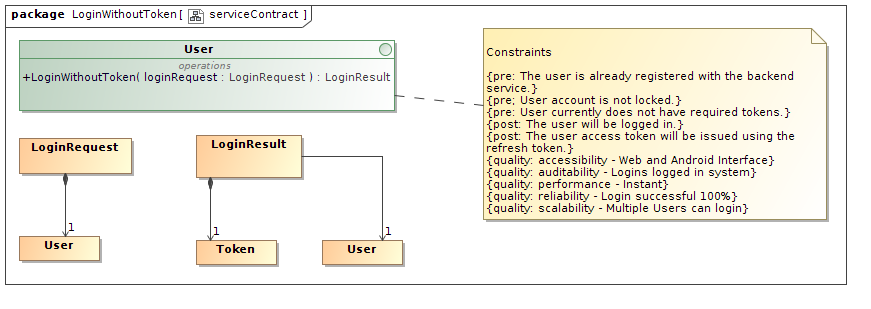
\includegraphics[scale=0.5]{loginWithoutToken}
				\caption{Login without Token Service Contract}
			\end{figure}
	\end{itemize}
	
\subsubsection{User Login - User holds access and refresh tokens}
	\begin{itemize}
		\item Description\\
		This use case will be used by the REST clients, specifically the Android app, to achieve safe long term login without storing user credentials on device. 
		\item Pre-Conditions
			\begin{enumerate}
				\item The user is already registered with the back-end service
				\item User account is not locked
				\item User currently has access and refresh tokens
			\end{enumerate}
		\item Post-Conditions
			\begin{enumerate}
				\item The user will be logged in
				\item The user access token will be updated using the refresh token
			\end{enumerate}
		\item Service Contract
			\begin{figure}[H]
				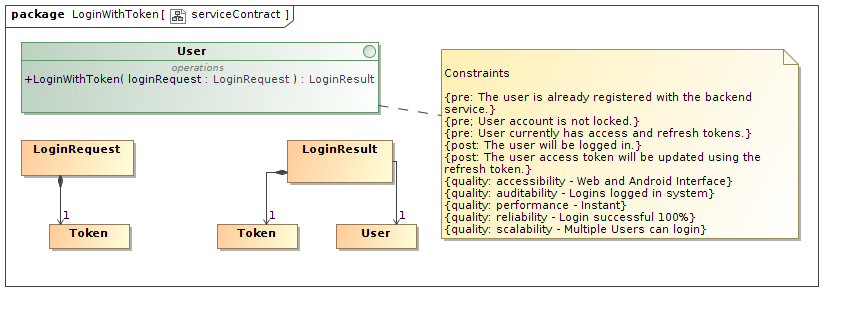
\includegraphics[scale=0.5]{loginWithToken}
				\caption{Login with Token Service Contract}
			\end{figure}
	\end{itemize}




\subsubsection{Log Out User}
	\begin{itemize}
		\item Description\\
			This use case will be used by the REST clients, specifically the web client and Android app, to log a user out of the system.
		\item Pre-Conditions
			\begin{enumerate}
				\item The user is currently logged into the system
			\end{enumerate}
		\item Post-Conditions
			\begin{enumerate}
				\item The user will be logged out of the system
						
			\end{enumerate}
		\item Service Contract
			\begin{figure}[H]
				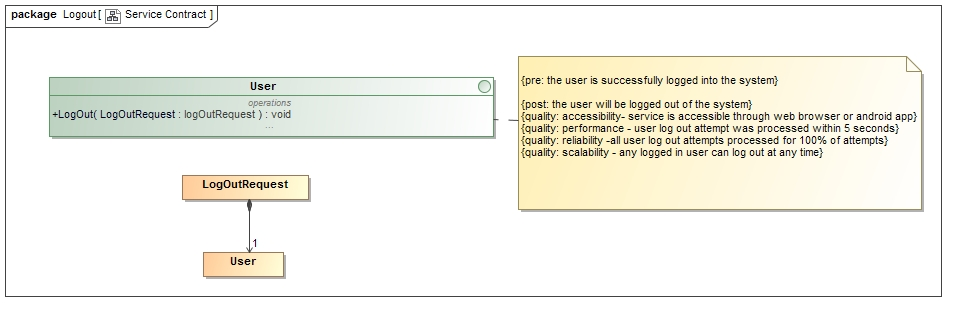
\includegraphics[scale=0.5]{Log_Out}
				\caption{Log the User out of the System}
			\end{figure}
	\end{itemize}

\subsubsection{Register User}
	\begin{itemize}
		\item Description\\
			This use case will be used by the REST clients, specifically the web client and Android app, to Create a user of the system.
		\item Pre-Conditions
			\begin{enumerate}
				\item The user does not exist in the system
				\item All required details have been provided
				\item All details are valid
			\end{enumerate}
		\item Post-Conditions
			\begin{enumerate}
				\item The user will be created in the database
						
			\end{enumerate}
		\item Service Contract
			\begin{figure}[H]
				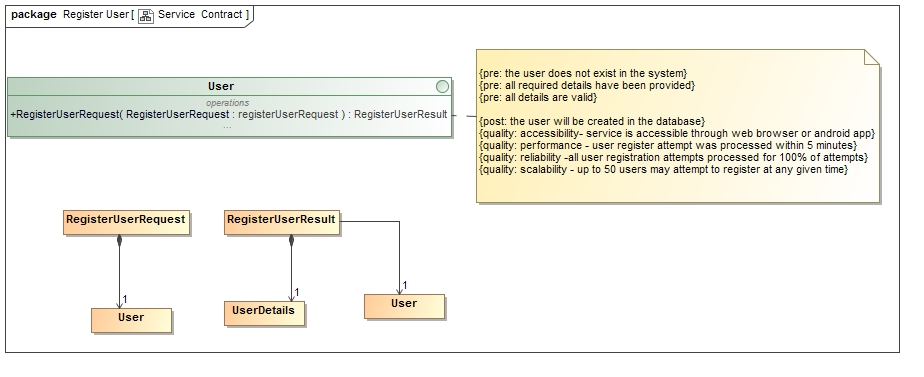
\includegraphics[scale=0.5]{Register_User}
				\caption{Register a User in the System}
			\end{figure}
	\end{itemize}
\subsubsection{View/Edit User}
	\begin{itemize}
		\item Description\\
			This use case will be used by the REST clients, specifically the web client and Android app, to View and Edit the currently logged in User.
		\item Pre-Conditions
			\begin{enumerate}
				\item The user is successfully logged in to the system
				\item Edited details are valid
			\end{enumerate}
		\item Post-Conditions
			\begin{enumerate}
				\item The user details will be edited
				\item All papers that the user is an author of should be displayed 
				\item User page will be displayed
						
			\end{enumerate}
		\item Service Contract
				\begin{figure}[H]
				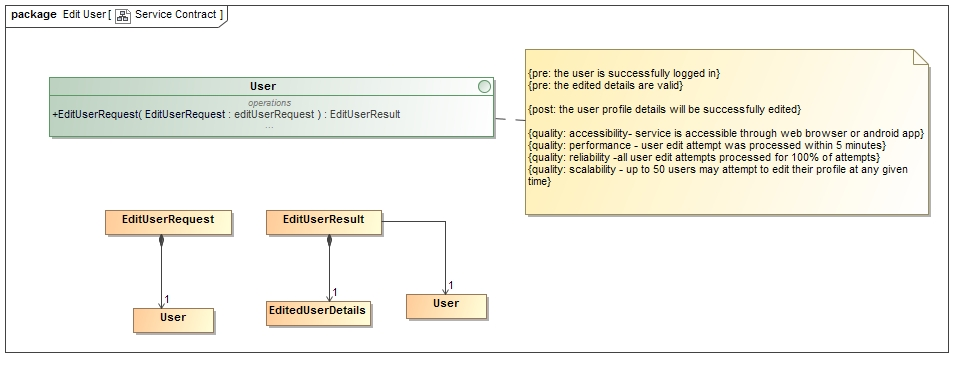
\includegraphics[scale=0.5]{Edit_User}
				\caption{Edit a User Profile in the System}	
				\end{figure}
	\end{itemize}

\subsubsection{Create Paper}
	\begin{itemize}
		\item Description\\
			This use case will be used by the REST clients, specifically the web client and Android app, to Create a Research Paper.
		\item Pre-Conditions
			\begin{enumerate}
				\item The user is successfully logged in to the system
				\item Paper details are filled in and valid
				\item The user must belong to a research group
			\end{enumerate}
		\item Post-Conditions
			\begin{enumerate}
				\item Paper successfully created

						
			\end{enumerate}
		\item Service Contract
			\begin{figure}[H]
				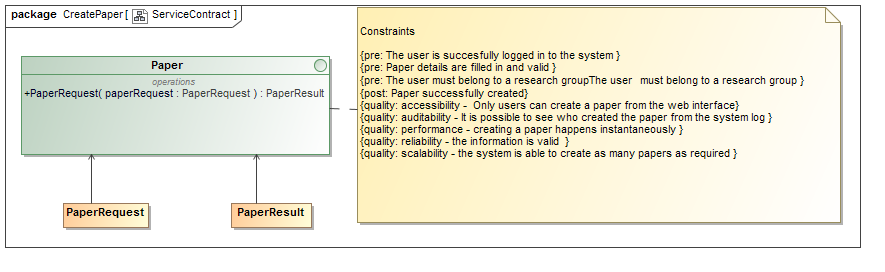
\includegraphics[scale=0.5]{CreatePaperServiceContract}
				\caption{Create Paper Service Contract}
			\end{figure}



	\end{itemize}

\subsubsection{Edit Paper}
	\begin{itemize}
		\item Description\\
			This use case will be used by the REST clients, specifically the web client and Android app, to Edit a Research Paper.
		\item Pre-Conditions
			\begin{enumerate}
				\item The user is successfully logged in to the system
				\item The user is an Author of the Paper
				\item The user is an HOD or a Research Group Leader for the Group of the Paper
				\item The new details are valid
			\end{enumerate}
		\item Post-Conditions
			\begin{enumerate}
				\item The paper's details will be edited
				\item The paper details will be displayed
						
			\end{enumerate}
		\item Service Contract
			\begin{figure}[H]
				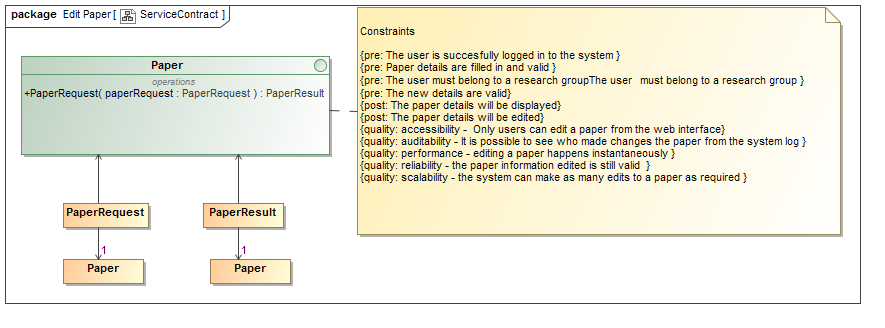
\includegraphics[scale=0.5]{EditPaperServiceContract}
				\caption{Edit Paper Service Contract}
			\end{figure}



	\end{itemize}

\subsubsection{View Paper}
	\begin{itemize}
		\item Description\\
			This use case will be used by the REST clients, specifically the web client and Android app, to View a Research Paper.
		\item Pre-Conditions
			\begin{enumerate}
				\item The user is successfully logged in to the system
				\item The user is an Author of the Paper
				\item The user is an HOD or a Research Group Leader for the Group of the Paper
			\end{enumerate}
		\item Post-Conditions
			\begin{enumerate}
				\item The paper details will be displayed
						
			\end{enumerate}
		\item Service Contract
			\begin{figure}[H]
				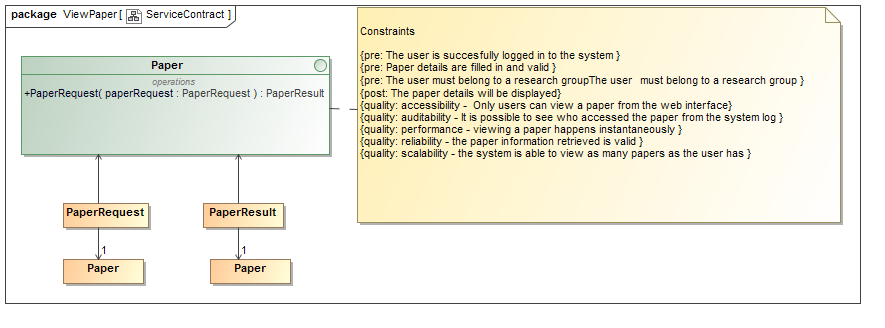
\includegraphics[scale=0.5]{ViewPaperServiceContract}
				\caption{View Paper Service Contract}
			\end{figure}

	\end{itemize}

\subsubsection{Create Author}
	\begin{itemize}
		\item Description\\
			This use case will be used by the REST clients, specifically the web client and Android app, to Create Authors.
		\item Pre-Conditions
			\begin{enumerate}
				\item The user is successfully logged in to the system
				\item The details for the Author are valid
				\item The author must not previously exist in the system 
			\end{enumerate}
		\item Post-Conditions
			\begin{enumerate}
				\item The Author is successfully created	
			\end{enumerate}
		\item Service Contract
			\begin{figure}[H]
				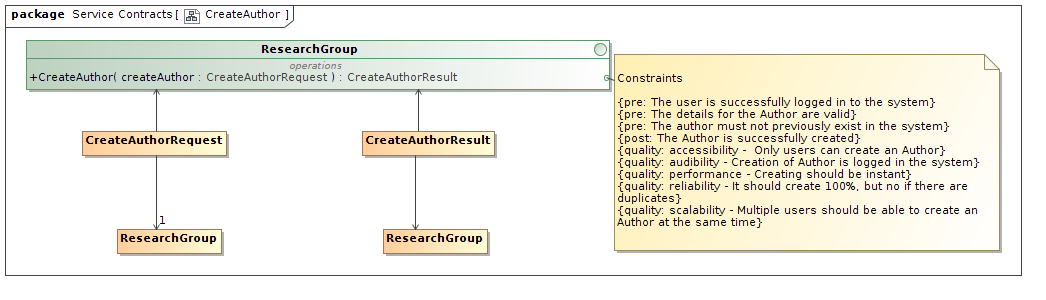
\includegraphics[scale=0.5]{CreateAuthor}
				\caption{Create Author}
			\end{figure}
	\end{itemize}

\subsubsection{View Author}
	\begin{itemize}
		\item Description\\
			This use case will be used by the REST clients, specifically the web client and Android app, to View an Author.
		\item Pre-Conditions
			\begin{enumerate}
				\item The user is successfully logged in to the system
			\end{enumerate}
		\item Post-Conditions
			\begin{enumerate}
				\item The Authors details will be displayed
						
			\end{enumerate}
		\item Service Contract
		\begin{figure}[H]
			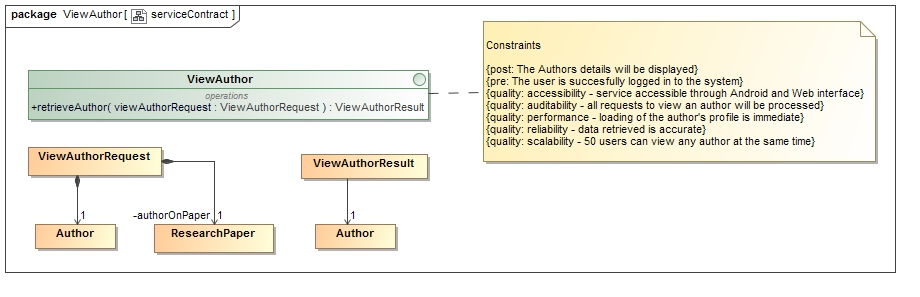
\includegraphics[scale=0.5]{ViewAuthorServiceContract}
			\caption{View author service contract}
		\end{figure}
	\end{itemize}
	
\subsubsection{Edit Author}
	\begin{itemize}
		\item Description\\
		This use case will be used by the REST clients, specifically the web client and Android app, to Edit an Author.
		\item Pre-Conditions
		\begin{enumerate}
			\item The user is successfully logged in to the system
			\item The new details are valid
		\end{enumerate}
		\item Post-Conditions
		\begin{enumerate}
			\item The Authors details will be edited
			\item The Authors details will be displayed
			
		\end{enumerate}
		\item Service Contract
		\begin{figure}[H]
			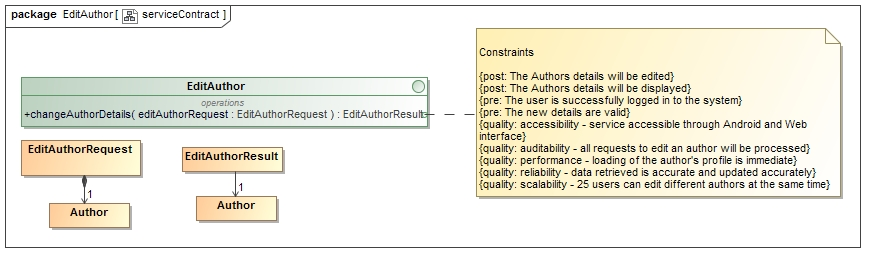
\includegraphics[scale=0.5]{EditAuthorServiceContract}
			\caption{Edit author service contract}
		\end{figure}
	\end{itemize}


\subsubsection{Add/Remove Author to Research Paper}
	\begin{itemize}
		\item Description\\
			This use case will be used by the REST clients, specifically the web client and Android app, to Add and Remove Authors of a Research Paper.
		\item Pre-Conditions
			\begin{enumerate}
				\item The user is successfully logged in to the system
				\item The user is an Author of the Paper
				\item The user is an HOD or a Research Group Leader for the Group of the Paper
				\item The new details are valid
			\end{enumerate}
		\item Post-Conditions
			\begin{enumerate}
				\item The Papers Authors have changed successfully
						
			\end{enumerate}
		\item Service Contract
			\begin{figure}[H]
				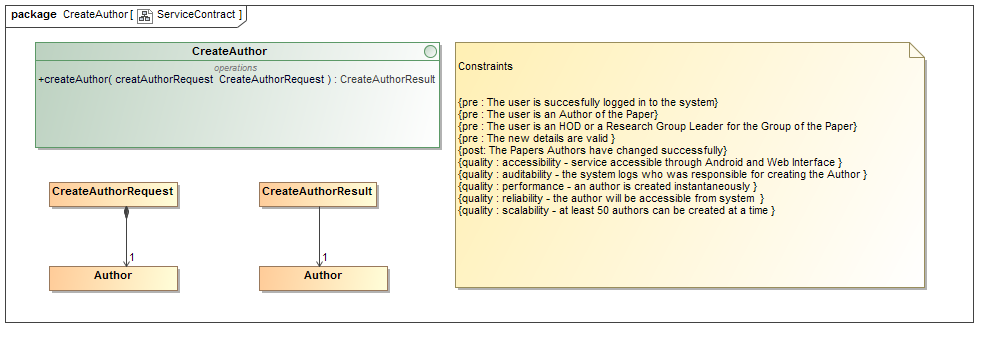
\includegraphics[scale=0.5]{CreateAuthorServiceContract}
				\caption{Create Author Service Contract}
			\end{figure}



	\end{itemize}

\subsubsection{Create Research Group}
	\begin{itemize}
		\item Description\\
			This use case will be used by the REST clients, specifically the web client and Android app, to Create a Research Group.
		\item Pre-Conditions
			\begin{enumerate}
				\item The user is successfully logged in to the system
				\item The user is an HOD or a Research Group Leader for the Group of the Paper
			\end{enumerate}
		\item Post-Conditions
			\begin{enumerate}
				\item The Research Group is successfully added
						
			\end{enumerate}
		\item Service Contract
			\begin{figure}[H]
				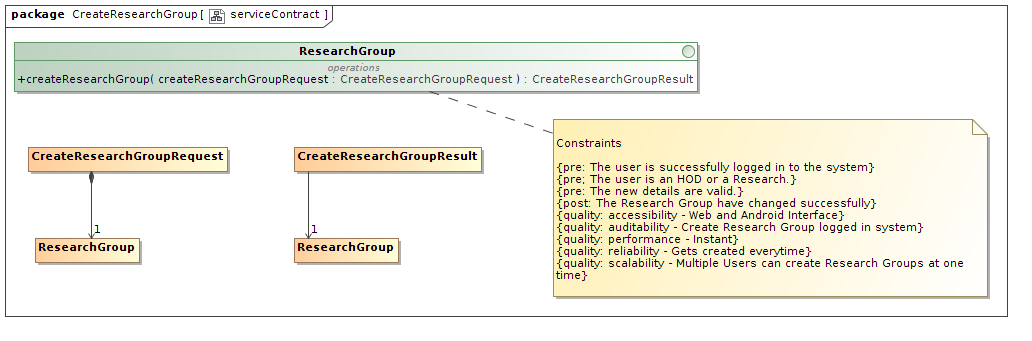
\includegraphics[scale=0.5]{createResearchGroup}
				\caption{Create Research Group Service Contract}
			\end{figure}
	\end{itemize}
	
	\subsubsection{View Research Groups}
	\begin{itemize}
		\item Description\\
		This use case will be used by the REST clients, specifically the web client and Android app, to View a Research Group.
		\item Pre-Conditions
		\begin{enumerate}
			\item The user is successfully logged in to the system
			\item The user is an HOD or a Research Group Leader for the Group of the Paper
		\end{enumerate}
		\item Post-Conditions
		\begin{enumerate}
			\item The Research Group has been displayed
			
		\end{enumerate}
		\item Service Contract
		\begin{figure}[H]
			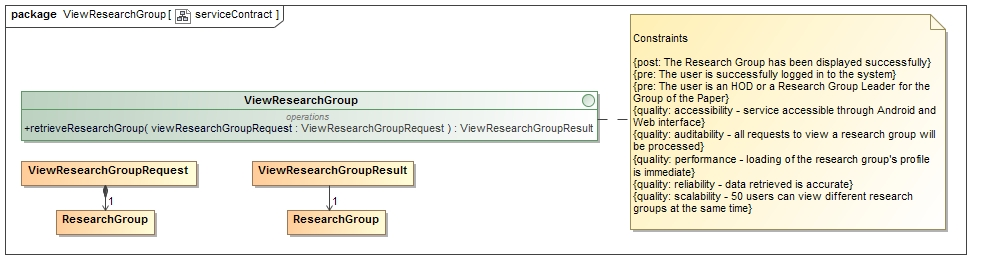
\includegraphics[scale=0.5]{ViewResearchGroupServiceContract}
			\caption{View research group service contract}
		\end{figure}
	\end{itemize}

\subsubsection{Edit Research Groups}
	\begin{itemize}
		\item Description\\
			This use case will be used by the REST clients, specifically the web client and Android app, to Edit a Research Group.
		\item Pre-Conditions
			\begin{enumerate}
				\item The user is successfully logged in to the system
				\item The user is an HOD or a Research Group Leader for the Group of the Paper
				\item The new details are valid
			\end{enumerate}
		\item Post-Conditions
			\begin{enumerate}
				\item The Research Group has been changed successfully
						
			\end{enumerate}
		\item Service Contract
			\begin{figure}[H]
				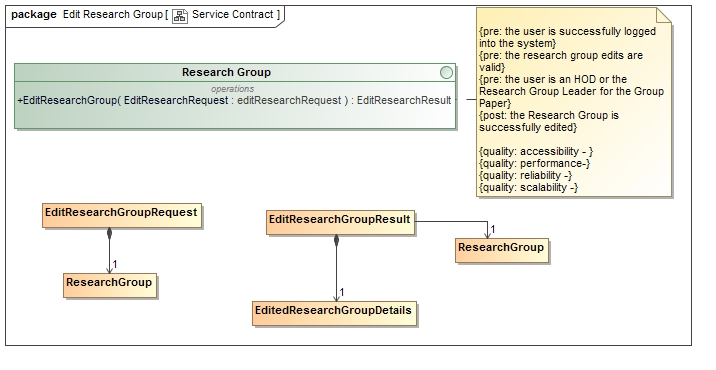
\includegraphics[scale=0.5]{Edit_Research_Group.jpg}
				\caption{Edit a Research Group's data in the System}
			\end{figure}
	\end{itemize}

\subsubsection{Add/Remove Users to Research Groups}
	\begin{itemize}
		\item Description\\
			This use case will be used by the REST clients, specifically the web client and Android app, to Add/Remove Users to a  Research Group.
		\item Pre-Conditions
			\begin{enumerate}
				\item The user is successfully logged in to the system
				\item The user is an HOD or a Research Group Leader for the Group of the Paper
				\item The user is valid
			\end{enumerate}
		\item Post-Conditions
			\begin{enumerate}
				\item The User is successfully added to a Research Group
						
			\end{enumerate}
		\item Service Contract
		\begin{figure}[H]
			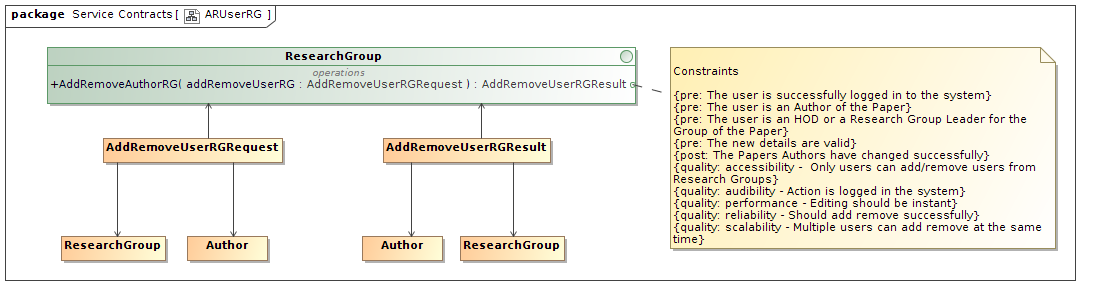
\includegraphics[scale=0.5]{ARUserRG}
			\caption{Add Users to Research Group}
		\end{figure}
	\end{itemize}

\subsubsection{Import Historical Paper}
	\begin{itemize}
		\item Description\\
			This use case will be used by the REST clients, specifically the web client and Android app, to Import a Historical Paper.
		\item Pre-Conditions
			\begin{enumerate}
				\item The user is successfully logged in to the system
				\item The paper details are correct
			\end{enumerate}
		\item Post-Conditions
			\begin{enumerate}
				\item The Historical Paper is successfully added
						
			\end{enumerate}
		\item Service Contract
		\begin{figure}[H]
			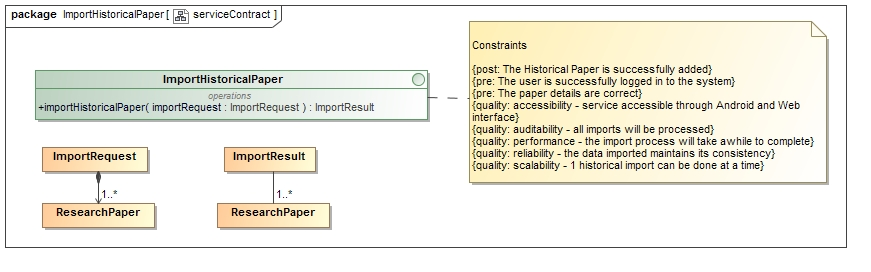
\includegraphics[scale=0.5]{ImportHistoricalPaperServiceContract}
			\caption{Import historical paper service contract}
		\end{figure}
	\end{itemize}

\subsubsection{Generate Bibliography}
	\begin{itemize}
		\item Description\\
			This use case will be used by the REST clients, specifically the web client and Android app, to Generate a Bibliography for a User.
		\item Pre-Conditions
			\begin{enumerate}
				\item The user is successfully logged in to the system
			\end{enumerate}
		\item Post-Conditions
			\begin{enumerate}
				\item Bibliography successfully generated
						
			\end{enumerate}
		\item Service Contract
			\begin{figure}[H]
				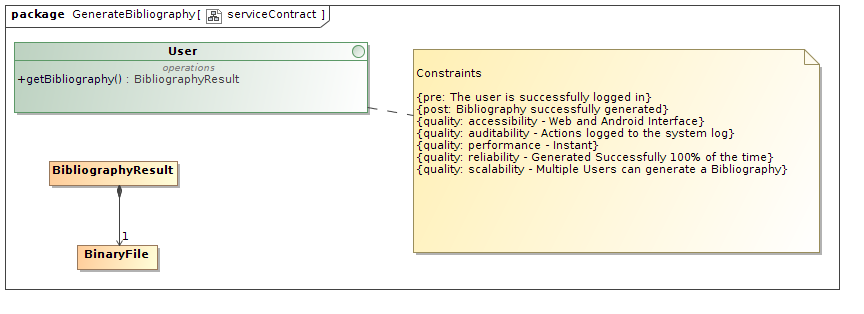
\includegraphics[scale=0.5]{generateBibliography}
				\caption{Generate Bibliography Service Contract}
			\end{figure}
	\end{itemize}


\subsubsection{Create Venue}
	\begin{itemize}
		\item Description\\
			This use case will be used by the REST clients, specifically the web client and Android app, to Create a Venue.
		\item Pre-Conditions
			\begin{enumerate}
				\item The user is successfully logged in to the system
				\item Venue details are valid
			\end{enumerate}
		\item Post-Conditions
			\begin{enumerate}
				\item The Venue is successfully created
						
			\end{enumerate}
		\item Service Contract
			\begin{figure}[H]
				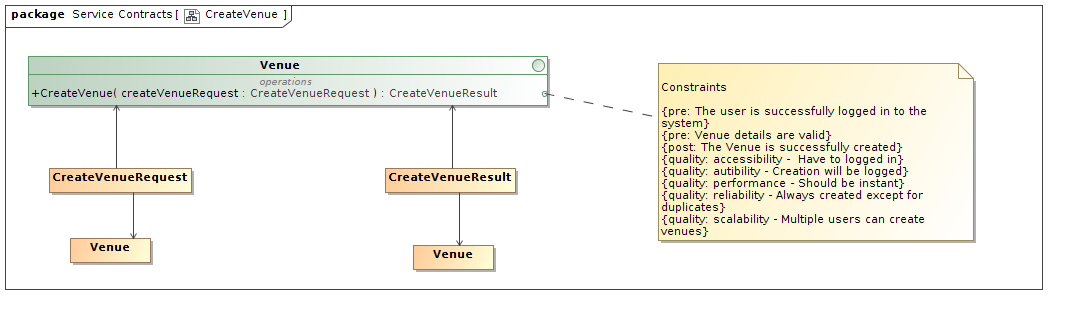
\includegraphics[scale=0.5]{CreateVenue}
				\caption{Create Venue}
			\end{figure}
	\end{itemize}

\subsubsection{View/Edit Venue}
	\begin{itemize}
		\item Description\\
			This use case will be used by the REST clients, specifically the web client and Android app, to View/Edit a Venue.
		\item Pre-Conditions
			\begin{enumerate}
				\item The user is successfully logged in to the system
				\item The new details are valid
			\end{enumerate}
		\item Post-Conditions
			\begin{enumerate}
				\item The Venue is successfully edited
						
			\end{enumerate}
		\item Service Contract
			\begin{figure}[H]
				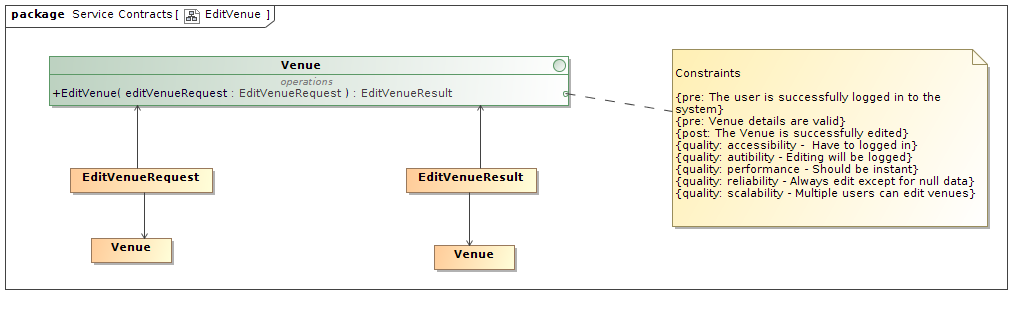
\includegraphics[scale=0.5]{EditVenue}
				\caption{View/Edit Venue}
			\end{figure}
	\end{itemize}


\subsubsection{View Log}
	\begin{itemize}
		\item Description\\
			This use case will be used by the REST clients, specifically the web client and Android app, to view a system log.
		\item Pre-Conditions
			\begin{enumerate}
				\item The user is successfully logged in to the system
				\item The user must be a Super User
			\end{enumerate}
		\item Post-Conditions
			\begin{enumerate}
				\item The system log will be displayed
				
						
			\end{enumerate}
	\end{itemize}



\subsection{Required functionality}

\subsubsection{Login with Token}
	\begin{figure}[H]
		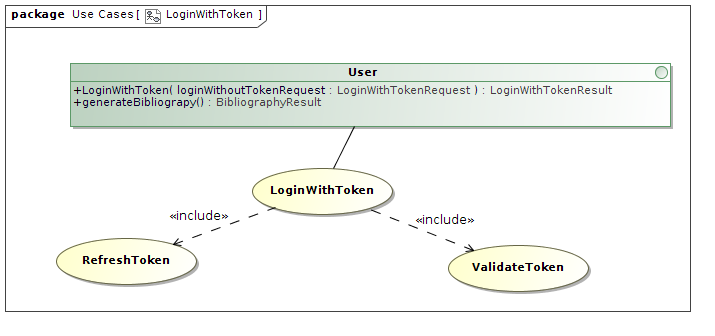
\includegraphics[scale=0.5]{LoginWithTokenUse}
	\caption{Use Case for Login with Token}
	\end{figure}

\subsubsection{Login without Token}
	\begin{figure}[H]
		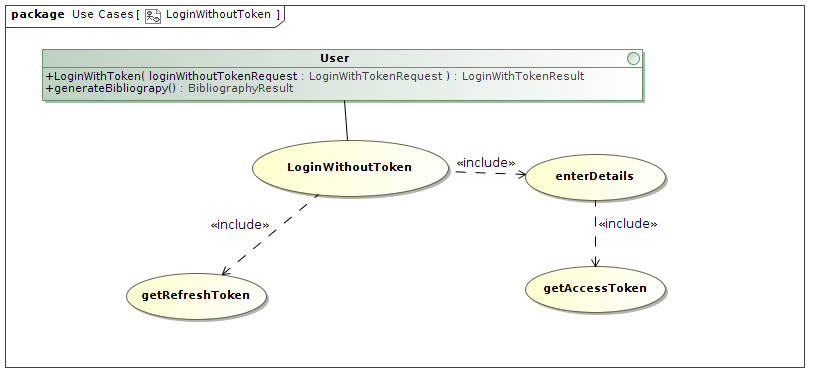
\includegraphics[scale=0.5]{LoginWithoutTokenUse}
	\caption{Use Case for Login without Token}
	\end{figure}

\subsubsection{Edit Research Group}
	\begin{figure}[H]
		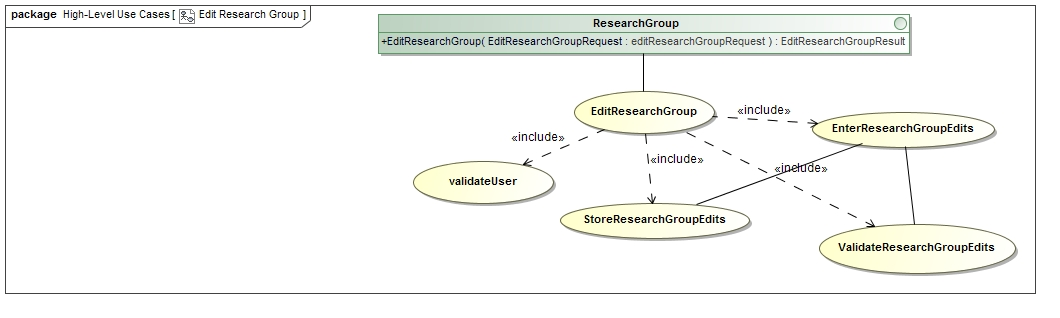
\includegraphics[scale=0.5]{UseEditResearchGroup}
	\caption{Use Case for Edit Research Group}
	\end{figure}
	
\subsubsection{Edit User}
	\begin{figure}[H]
		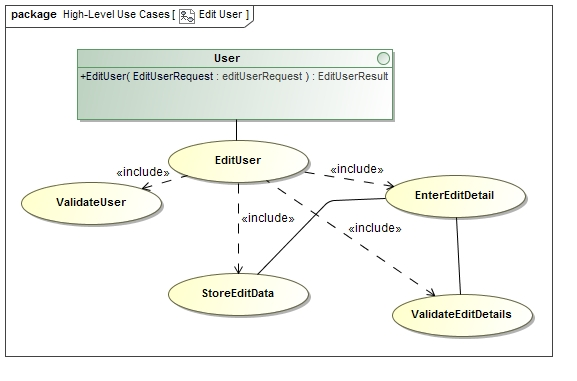
\includegraphics[scale=0.5]{UseEditUser}
	\caption{Use Case for Edit User}
	\end{figure}
		
\subsubsection{View User}
	\begin{figure}[H]
		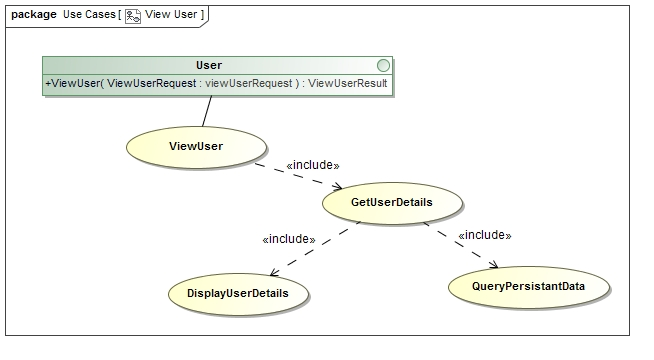
\includegraphics[scale=0.5]{UseViewUser}
	\caption{Use Case for View User}
	\end{figure}
		
\subsubsection{User Log Out}
	\begin{figure}[H]
		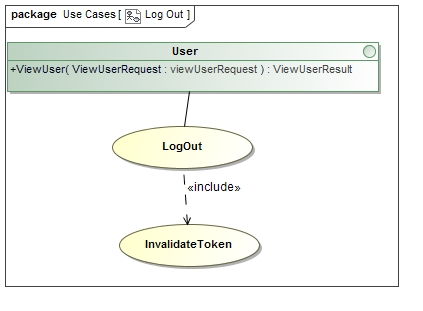
\includegraphics[scale=0.5]{UseLogOut}
	\caption{Use Case for User Log Out}
	\end{figure}
	
\subsubsection{Create Paper}
	\begin{figure}[H]
		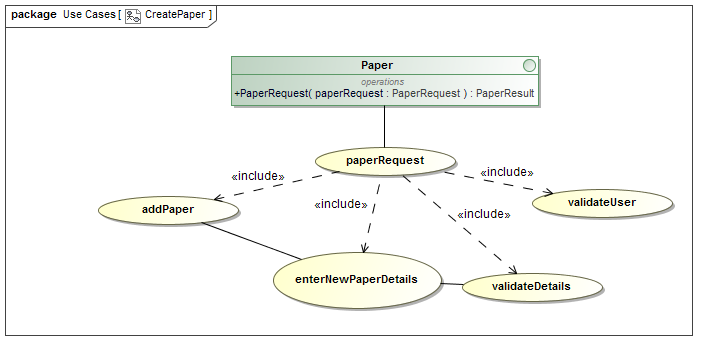
\includegraphics[scale=0.5]{Use_CreatePaper}
	\caption{Use Case for Create Paper}
	\end{figure}


\subsubsection{View Paper}
	\begin{figure}[H]
		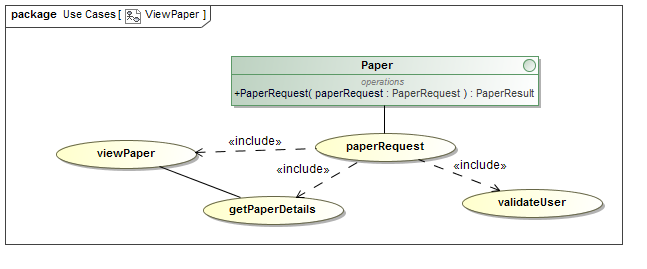
\includegraphics[scale=0.5]{Use_ViewPaper}
	\caption{Use Case for View Paper}
	\end{figure}

\subsubsection{Edit Paper}
	\begin{figure}[H]
		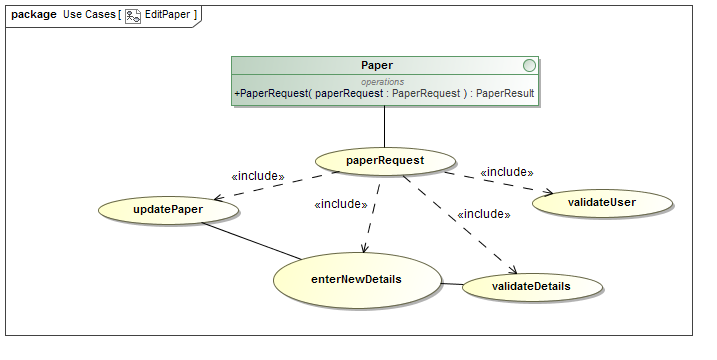
\includegraphics[scale=0.5]{Use_EditPaper}
	\caption{Use Case for Edit Paper}
	\end{figure}
	
\subsubsection{Register User}
	\begin{figure}[H]
		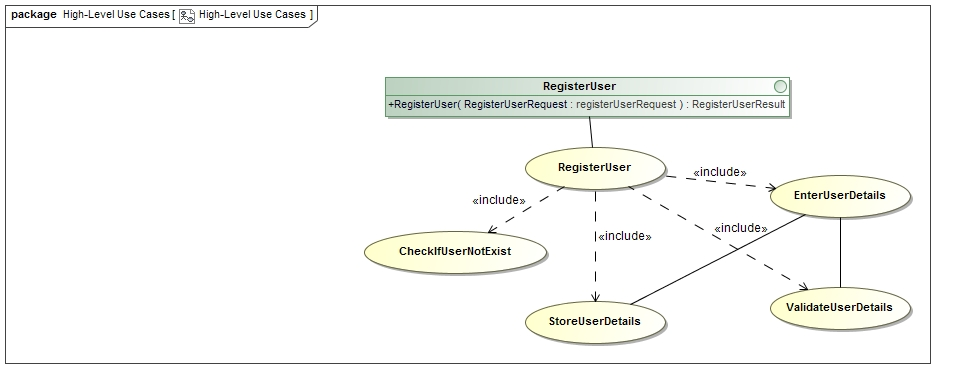
\includegraphics[scale=0.5]{UseRegisterUser}
	\caption{Use Case for Register User}
	\end{figure}

\subsubsection{Create Author}
	\begin{figure}[H]
		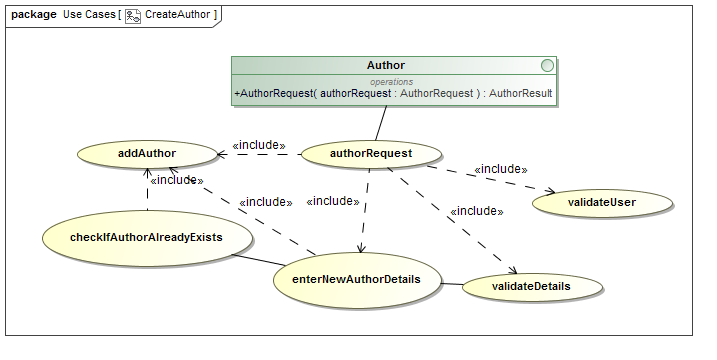
\includegraphics[scale=0.5]{Use_CreateAuthor}
		\caption{Use Case Diagram for Create Author}
	\end{figure}
	
\subsubsection{View Author}
	\begin{figure}[H]
		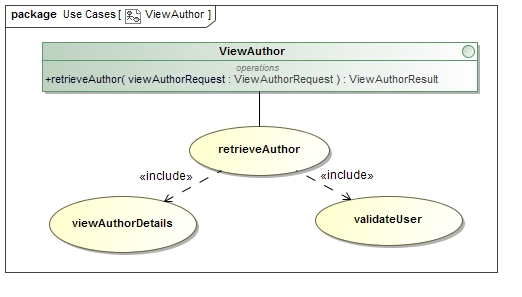
\includegraphics[scale=0.5]{UseViewAuthor}
		\caption{Use Case Diagram for View Author}
	\end{figure}
	
\subsubsection{Edit Author}
	\begin{figure}[H]
		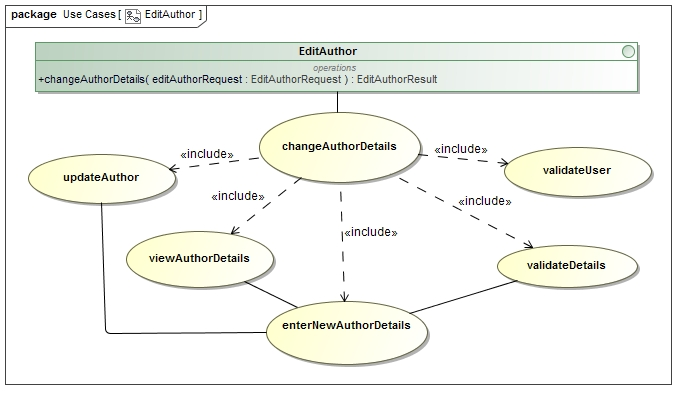
\includegraphics[scale=0.5]{UseEditAuthor}
		\caption{Use Case Diagram for Edit User}
	\end{figure}

\subsubsection{Create Research Group}
	\begin{figure}[H]
		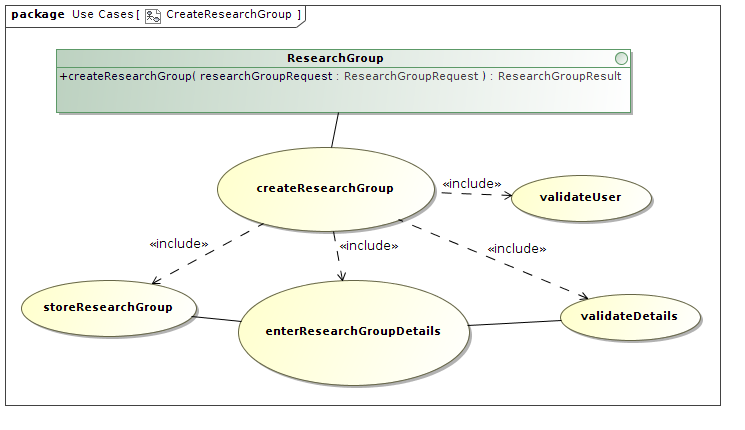
\includegraphics[scale=0.5]{CreateResearchGroupUse}
	\caption{Use Case for Creating a Research Group}
	\end{figure}
	
\subsubsection{View Research Group}
	\begin{figure}[H]
		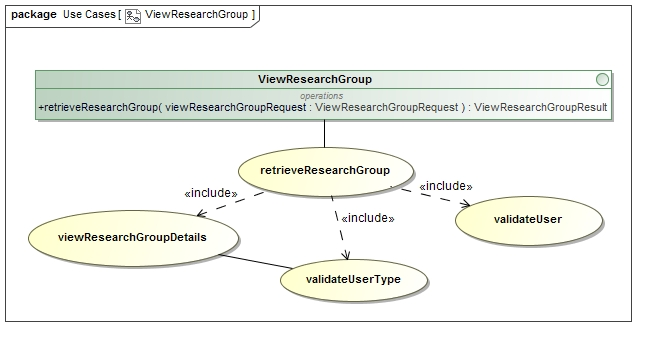
\includegraphics[scale=0.5]{UseViewResearchGroup}
		\caption{Use Case Diagram for View Research Group}
	\end{figure}
	
\subsubsection{Import Historical Paper}
	\begin{figure}[H]
		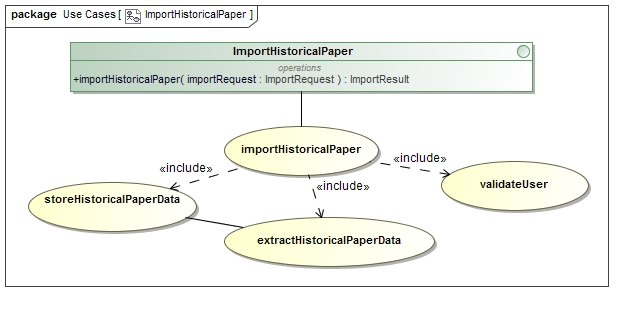
\includegraphics[scale=0.5]{UseImportHistoricalPaper}
		\caption{Use Case Diagram for Import Historical Paper}
	\end{figure}

\subsubsection{Generate Bibliography}
	\begin{figure}[H]
		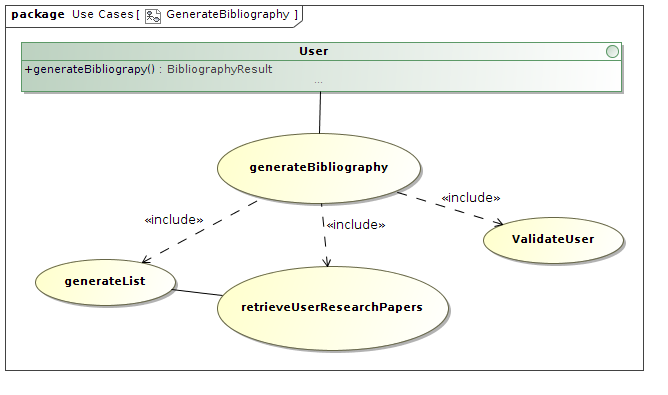
\includegraphics[scale=0.5]{GenerateBibliographyUse}
	\caption{Use Case for Generating a Bibliography}
	\end{figure}






\subsection{Process specifications}

\subsubsection{Login with Token}
	\begin{figure}[H]
		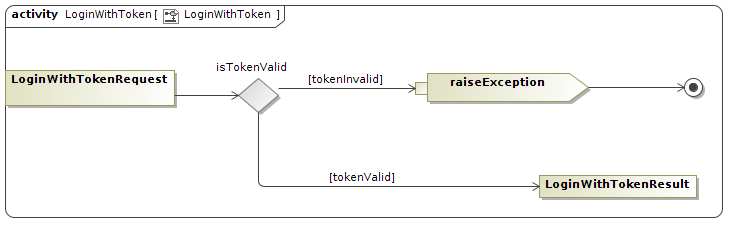
\includegraphics[scale=0.5]{LoginWithTokenAct}
	\caption{Activity Diagram for Login with Token}
	\end{figure}

\subsubsection{Login without Token}
	\begin{figure}[H]
		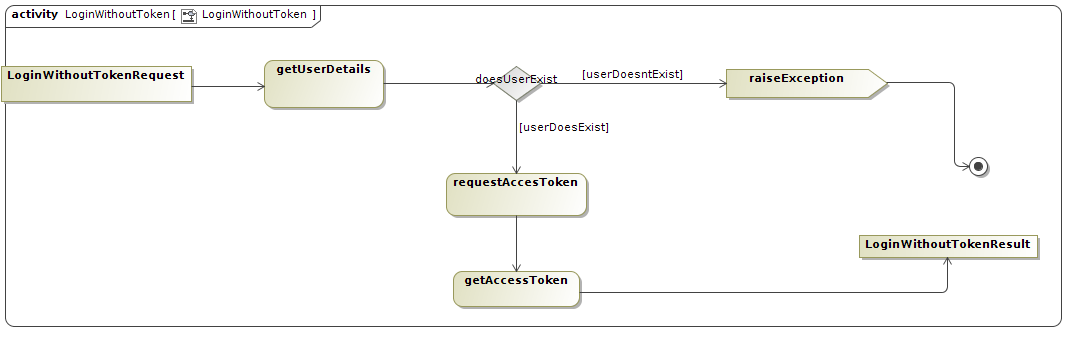
\includegraphics[scale=0.5]{LoginWithoutTokenAct}
	\caption{Activity Diagram for Login without Token}
	\end{figure}

\subsubsection{Edit Research}
	\begin{figure}[H]
	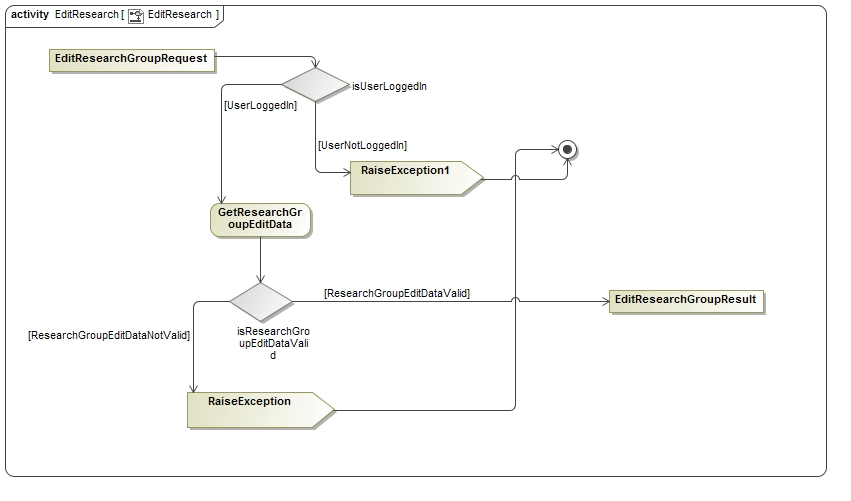
\includegraphics[scale=0.5]{ActEditResearch}
	\caption{Process Specification for Edit Research}
	\end{figure}
	
\subsubsection{Edit User}
	\begin{figure}[H]
	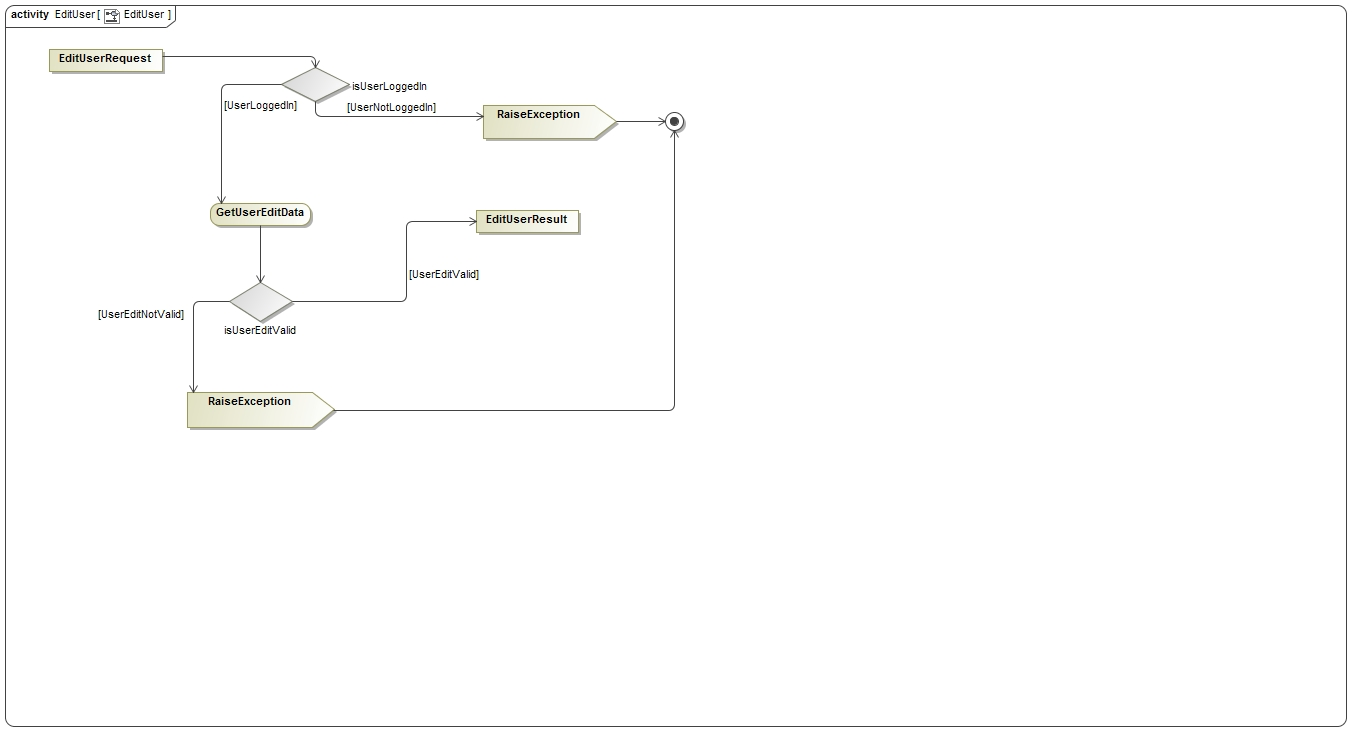
\includegraphics[scale=0.5]{ActEditUser}
	\caption{Process Specification for Edit User}
	\end{figure}
		
\subsubsection{Log Out}
	\begin{figure}[H]
	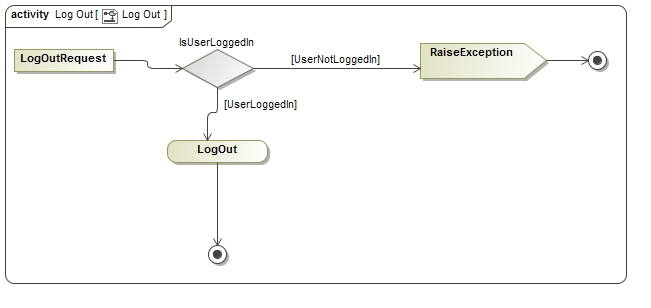
\includegraphics[scale=0.5]{ActLogOut}
	\caption{Process Specification for Log Out}
	\end{figure}
		
\subsubsection{Register User}
	\begin{figure}[H]
	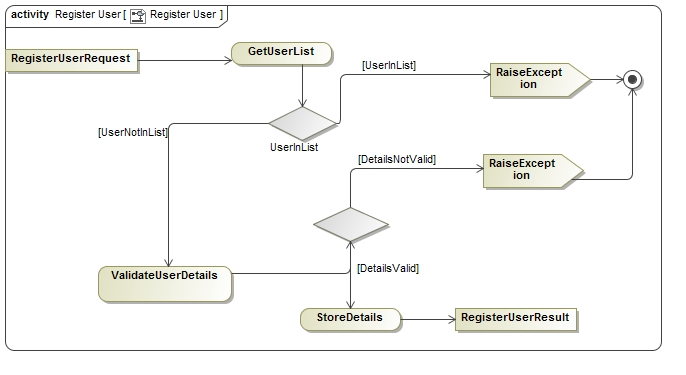
\includegraphics[scale=0.5]{ActRegisterUser}
	\caption{Process Specification for Register User}
	\end{figure}
		
\subsubsection{View User}
	\begin{figure}[H]
	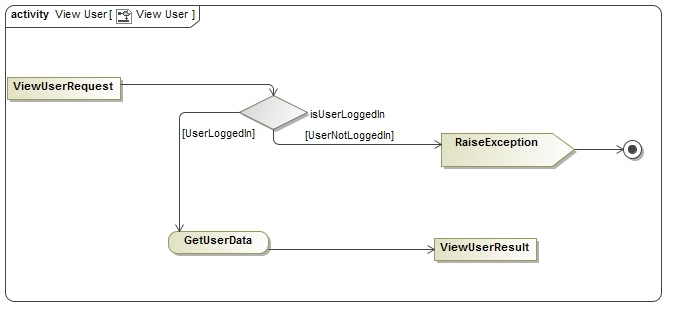
\includegraphics[scale=0.5]{ActViewUser}
	\caption{Process Specification for View User}
	\end{figure}
	
\subsubsection{View Author}
	\begin{figure}[H]
		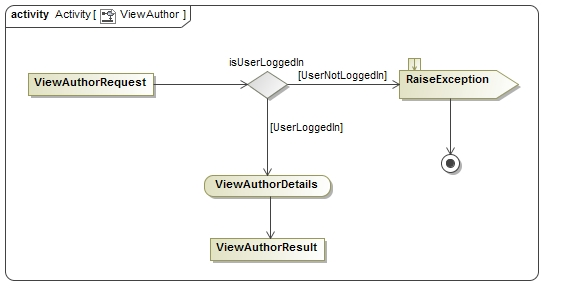
\includegraphics[scale=0.5]{ActViewAuthor}
		\caption{Activity Diagram for View Author}
	\end{figure}

\subsubsection{Create Author}
	\begin{figure}[H]
		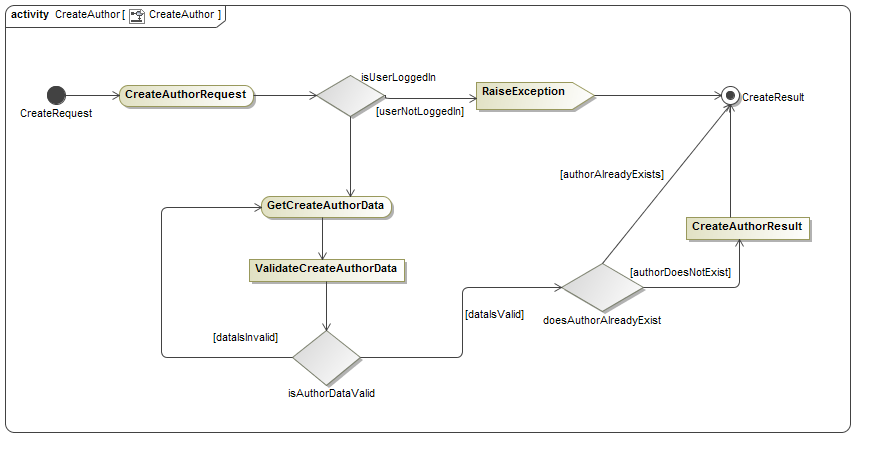
\includegraphics[scale=0.5]{Activity_CreateAuthor}
		\caption{Activity Diagram for Create Author}
	\end{figure}

	
\subsubsection{Edit Author}
	\begin{figure}[H]
		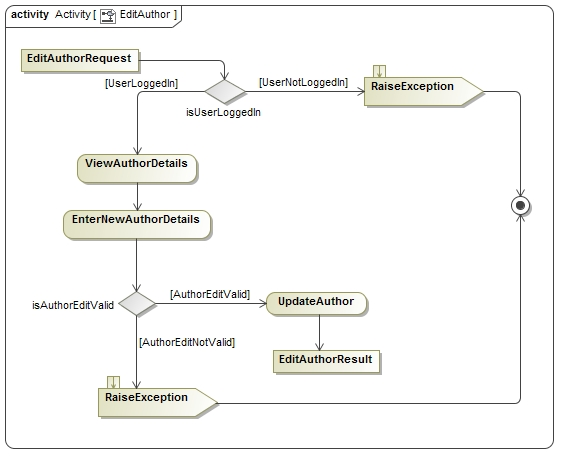
\includegraphics[scale=0.5]{ActEditAuthor}
		\caption{Activity Diagram for Edit User}
	\end{figure}

\subsubsection{Create Research Group}
	\begin{figure}[H]
		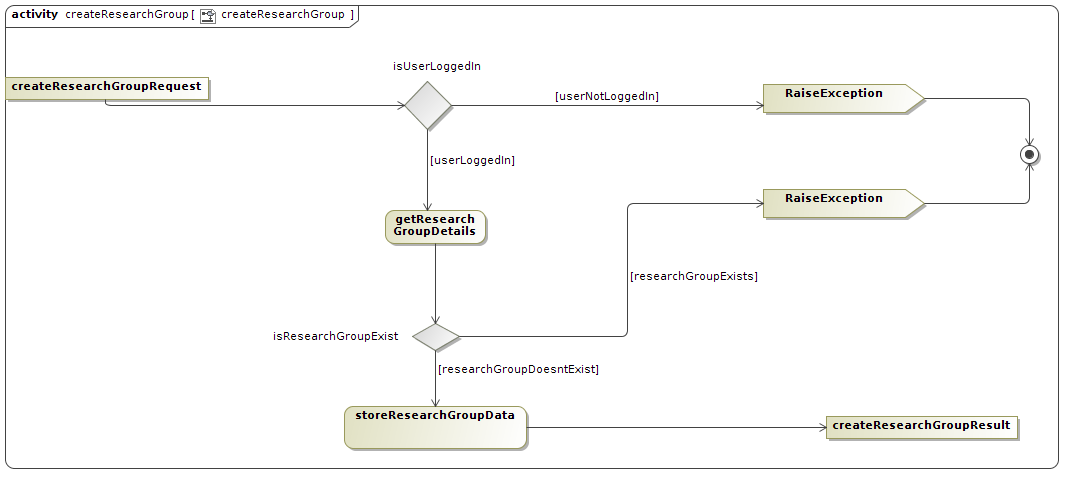
\includegraphics[scale=0.5]{createResearchGroupAct}
	\caption{Activity Diagram for Creating a Research Group}
	\end{figure}

\subsubsection{View Research Group}
	\begin{figure}[H]
		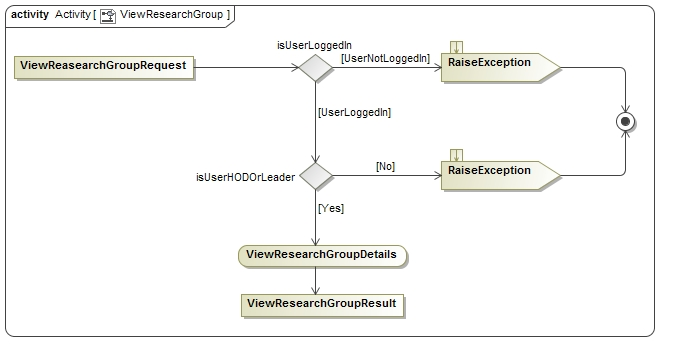
\includegraphics[scale=0.5]{ActViewResearchGroup}
		\caption{Activity Diagram for View Research Group}
	\end{figure}
	
\subsubsection{Import Historical Paper}
	\begin{figure}[H]
		\includegraphics[scale=0.5]{ActImportHistoricalPaper}
		\caption{Activity Diagram for Import Historical Paper}
	\end{figure}

	\subsubsection{Create Paper}
	\begin{figure}[H]
		\includegraphics[scale=0.5]{Activity_CreatePaper}
		\caption{Activity Diagram for Create Paper}
	\end{figure}

\subsubsection{View Paper}
	\begin{figure}[H]
		\includegraphics[scale=0.5]{Activity_ViewPaper}
		\caption{Activity Diagram for View Paper}
	\end{figure}

\subsubsection{Edit Paper}
	\begin{figure}[H]
		\includegraphics[scale=0.5]{Activity_EditPaper}
		\caption{Activity Diagram for Edit Paper}
	\end{figure}

\subsubsection{Generate Bibliography}
	\begin{figure}[H]
		\includegraphics[scale=0.5]{generateBibliographyAct}
	\caption{Activity Diagram for Generating a Bibliography}
	\end{figure}

	
	
\subsection{Domain Model}
	\begin{figure}[H]
		\includegraphics[width=7in]{DomainModel}
	\caption{Domain Model}
	\end{figure}
\section{Open Issues}
\subsection {GitHub Repository}
Team Echo Repository: \url{https://github.com/andrewbroekman/echo}

This repository contains:
\begin{enumerate}
\item All work done by team members.
\item \href{https://github.com/andrewbroekman/echo/blob/master/CONTRIBUTORS.md}{CONTRIBUTORS.md} file outlining which members where involved in which phases of the project.
\end{enumerate}

\begin{appendices}
\newpage
\section{Data Dictionary}
\begin{tabu} to \textwidth { | X[l] | X[l] | }
	\hline
		\textbf{Term}		& \textbf{Definition}	\\ \hline \hline
		Android			&  A Linux based operating system developed by Google Inc. and the Open Handset Alliance for smart phones, tablets, and other mobile computing devices. Android applications are developed in Java. \\ \hline
		HTTP			& HyperText Transfer Protocol, standardised by RFCs 7230-7237 \\ \hline
		ISO				& International Organization for Standardization \\ \hline
		MVC				& Model-View-Controller \\ \hline
		OAuth			& An open standard for authorization, using an access token approach, allowing resource owners to authorize third-party clients to access protected user resources on a resource server, without the client providing their credentials to the third-party in question. \\ \hline
		RDBMS			& Relational Database Management System \\ \hline
		SPA				& Single Page Application \\ \hline
		SQL				& Structured Query Language is a programming language, standardised by ISO for managing data in RDBMS. Actions allow for the creation, reading/retrieving, updating and deletion of data in the management system. \\ \hline
	\hline
\end{tabu}

\end{appendices}

\newpage
\clearpage
\addcontentsline{toc}{section}{References}
\printbibliography
\listoffigures



\end{document}
